\chapter{Case study: data structure selection}

\section{Word frequency analysis}
\label{analysis}

As usual, you should at least attempt the following exercises
before you read my solutions.

\begin{ex}
Write a program that reads a file, breaks each line into
words, strips whitespace and punctuation from the words, and
converts them to lowercase.

\index{string module}
\index{module!string}

Hint: The {\tt string} module provides strings named {\tt whitespace},
which contains space, tab, newline, etc., and {\tt
  punctuation} which contains the punctuation characters.  Let's see
if we can make Python swear:

\beforeverb
\begin{verbatim}
>>> import string
>>> print string.punctuation
!"#$%&'()*+,-./:;<=>?@[\]^_`{|}~
\end{verbatim}
\afterverb
%
Also, you might consider using the string methods {\tt strip},
{\tt replace} and {\tt translate}.

\index{strip method}
\index{method!strip}
\index{replace method}
\index{method!replace}
\index{translate method}
\index{method!translate}

\end{ex}


\begin{ex}

\index{Project Gutenberg}

Go to Project Gutenberg (\url{gutenberg.net}) and download 
your favorite out-of-copyright book in plain text format.

\index{plain text}
\index{text!plain}

Modify your program from the previous exercise to read the book
you downloaded, skip over the header information at the beginning
of the file, and process the rest of the words as before.

Then modify the program to count the total number of words in
the book, and the number of times each word is used.

\index{word frequency}
\index{frequency!word}

Print the number of different words used in the book.  Compare
different books by different authors, written in different eras.
Which author uses the most extensive vocabulary?
\end{ex}


\begin{ex}
Modify the program from the previous exercise to print the
20 most frequently-used words in the book.
\end{ex}


\begin{ex}
Modify the previous program to read a word list (see
Section~\ref{wordlist}) and then print all the words in the book that
are not in the word list.  How many of them are typos?  How many of
them are common words that {\em should} be in the word list, and how
many of them are really obscure?
\end{ex}


\section{Random numbers}

\index{random number}
\index{number, random}
\index{deterministic}
\index{pseudorandom}

Given the same inputs, most computer programs generate the same
outputs every time, so they are said to be {\bf deterministic}.
Determinism is usually a good thing, since we expect the same
calculation to yield the same result.  For some applications, though,
we want the computer to be unpredictable.  Games are an obvious
example, but there are more.

Making a program truly nondeterministic turns out to be not so easy,
but there are ways to make it at least seem nondeterministic.  One of
them is to use algorithms that generate {\bf pseudorandom} numbers.
Pseudorandom numbers are not truly random because they are generated
by a deterministic computation, but just by looking at the numbers it
is all but impossible to distinguish them from random.

\index{random module}
\index{module!random}

The {\tt random} module provides functions that generate
pseudorandom numbers (which I will simply call ``random'' from
here on).

\index{random function}
\index{function!random}

The function {\tt random} returns a random float
between 0.0 and 1.0 (including 0.0 but not 1.0).  Each time you
call {\tt random}, you get the next number in a long series.  To see a
sample, run this loop:

\beforeverb
\begin{verbatim}
import random

for i in range(10):
    x = random.random()
    print x
\end{verbatim}
\afterverb
%
The function {\tt randint} takes parameters {\tt low} and
{\tt high} and returns an integer between {\tt low} and
{\tt high} (including both).

\index{randint function}
\index{function!randint}

\beforeverb
\begin{verbatim}
>>> random.randint(5, 10)
5
>>> random.randint(5, 10)
9
\end{verbatim}
\afterverb
%
To choose an element from a sequence at random, you can use
{\tt choice}:

\index{choice function}
\index{function!choice}

\beforeverb
\begin{verbatim}
>>> t = [1, 2, 3]
>>> random.choice(t)
2
>>> random.choice(t)
3
\end{verbatim}
\afterverb
%
The {\tt random} module also provides functions to generate
random values from continuous distributions including
Gaussian, exponential, gamma, and a few more.

\begin{ex}

\index{histogram!random choice}

Write a function named \verb"choose_from_hist" that takes
a histogram as defined in Section~\ref{histogram} and returns a 
random value from the histogram, chosen with probability
in proportion to frequency.  For example, for this histogram:

\beforeverb
\begin{verbatim}
>>> t = ['a', 'a', 'b']
>>> h = histogram(t)
>>> print h
{'a': 2, 'b': 1}
\end{verbatim}
\afterverb
%
your function should {\tt 'a'} with probability $2/3$ and \verb"'b'"
with probability $1/3$.
\end{ex}


\section{Word histogram}

Here is a program that reads a file and builds a histogram of the
words in the file:

\index{histogram!word frequencies}

\beforeverb
\begin{verbatim}
import string

def process_file(filename):
    h = dict()
    fp = open(filename)
    for line in fp:
        process_line(line, h)
    return h

def process_line(line, h):
    line = line.replace('-', ' ')
    
    for word in line.split():
        word = word.strip(string.punctuation + string.whitespace)
        word = word.lower()

        h[word] = h.get(word, 0) + 1

hist = process_file('emma.txt')
\end{verbatim}
\afterverb
%
This program reads {\tt emma.txt}, which contains the text of {\em
  Emma} by Jane Austen.

\index{Austin, Jane}

\verb"process_file" loops through the lines of the file,
passing them one at a time to \verb"process_line".  The histogram
{\tt h} is being used as an accumulator.

\index{accumulator!histogram}
\index{traversal}

\verb"process_line" uses the string method {\tt replace} to replace
hyphens with spaces before using {\tt split} to break the line into a
list of strings.  It traverses the list of words and uses {\tt strip}
and {\tt lower} to remove punctuation and convert to lower case.  (It
is a shorthand to say that strings are ``converted;'' remember that
string are immutable, so methods like {\tt strip} and {\tt lower}
return new strings.)

Finally, \verb"process_line" updates the histogram by creating a new
item or incrementing an existing one.

\index{update!histogram}

To count the total number of words in the file, we can add up
the frequencies in the histogram:

\beforeverb
\begin{verbatim}
def total_words(h):
    return sum(h.values())
\end{verbatim}
\afterverb
%
The number of different words is just the number of items in
the dictionary:

\beforeverb
\begin{verbatim}
def different_words(h):
    return len(h)
\end{verbatim}
\afterverb
%
Here is some code to print the results:

\beforeverb
\begin{verbatim}
print 'Total number of words:', total_words(hist)
print 'Number of different words:', different_words(hist)
\end{verbatim}
\afterverb
%
And the results:

\beforeverb
\begin{verbatim}
Total number of words: 161073
Number of different words: 7212
\end{verbatim}
\afterverb
%

\section{Most common words}

\index{DSU pattern}
\index{pattern!DSU}

To find the most common words, we can apply the DSU pattern;
\verb"most_common" takes a histogram and returns a list of
word-frequency tuples, sorted in reverse order by frequency:

\beforeverb
\begin{verbatim}
def most_common(h):
    t = []
    for key, value in h.items():
        t.append((value, key))

    t.sort(reverse=True)
    return t
\end{verbatim}
\afterverb
%
Here is a loop that prints the ten most common words:

\beforeverb
\begin{verbatim}
t = most_common(hist)
print 'The most common words are:'
for freq, word in t[0:10]:
    print word, '\t', freq
\end{verbatim}
\afterverb
%
And here are the results from {\em Emma}:

\beforeverb
\begin{verbatim}
The most common words are:
to      5242
the     5204
and     4897
of      4293
i       3191
a       3130
it      2529
her     2483
was     2400
she     2364
\end{verbatim}
\afterverb
%

\section{Optional parameters}

\index{optional parameter}
\index{parameter!optional}

We have seen built-in functions and methods that take a variable
number of arguments.  It is possible to write user-defined functions
with optional arguments, too.  For example, here is a function that
prints the most common words in a histogram

\beforeverb
\begin{verbatim}
def print_most_common(hist, num=10)
    t = most_common(hist)
    print 'The most common words are:'
    for freq, word in t[0:num]:
        print word, '\t', freq
\end{verbatim}
\afterverb

The first parameter is required; the second is optional.
The {\bf default value} of {\tt num} is 10.

\index{default value}
\index{value!default}

If you only provide one argument:

\beforeverb
\begin{verbatim}
print_most_common(hist)
\end{verbatim}
\afterverb

{\tt num} gets the default value.  If you provide two arguments:

\beforeverb
\begin{verbatim}
print_most_common(hist, 20)
\end{verbatim}
\afterverb

{\tt num} gets the value of the argument instead.  In other
words, the optional argument {\bf overrides} the default value.

\index{override}

If a function has both required and optional parameters, all
the required parameters have to come first, followed by the
optional ones.


\section{Dictionary subtraction}

\index{dictionary!subtraction}
\index{subtraction!dictionary}

Finding the words from the book that are not in the word list
from {\tt words.txt} is a problem you might recognize as set
subtraction; that is, we want to find all the words from one
set (the words in the book) that are not in another set (the
words in the list).

{\tt subtract} takes dictionaries {\tt d1} and {\tt d2} and returns a
new dictionary that contains all the keys from {\tt d1} that are not
in {\tt d2}.  Since we don't really care about the values, we
set them all to None.

\beforeverb
\begin{verbatim}
def subtract(d1, d2):
    res = dict()
    for key in d1:
        if key not in d2:
            res[key] = None
    return res
\end{verbatim}
\afterverb
%
To find the words in the book that are not in {\tt words.txt},
we can use \verb"process_file" to build a histogram for
{\tt words.txt}, and then subtract:

\beforeverb
\begin{verbatim}
words = process_file('words.txt')
diff = subtract(hist, words)

print "The words in the book that aren't in the word list are:"
for word in diff.keys():
    print word,
\end{verbatim}
\afterverb
%
Here are some of the results from {\em Emma}:

\beforeverb
\begin{verbatim}
The words in the book that aren't in the word list are:
 rencontre jane's blanche woodhouses disingenuousness 
friend's venice apartment ...
\end{verbatim}
\afterverb
%
Some of these words are names and possessives.  Others, like
``rencontre,'' are no longer in common use.  But a few are common
words that should really be in the list!

\begin{ex}

\index{set}
\index{type!set}

Python provides a data structure called {\tt set} that provides many
common set operations.  Read the documentation at
\url{docs.python.org/lib/types-set.html} and write a program
that uses set subtraction to find words in the book that are not in
the word list.
\end{ex}


\section{Random words}
\label{randomwords}

\index{histogram!random choice}

To choose a random word from the histogram, the simplest algorithm
is to build a list with multiple copies of each word, according
to the observed frequency, and then choose from the list:

\beforeverb
\begin{verbatim}
def random_word(h):
    t = []
    for word, freq in h.items():
        t.extend([word] * freq)

    return random.choice(t)
\end{verbatim}
\afterverb
%
The expression {\tt [word] * freq} creates a list with {\tt freq}
copies of the string {\tt word}.  The {\tt extend}
method is similar to {\tt append} except that the argument is
a sequence.

\begin{ex}
\label{randhist}

\index{algorithm}

This algorithm works, but it is not very efficient; each time you
choose a random word, it rebuilds the list, which is as big as
the original book.  An obvious improvement is to build the list
once and then make multiple selections, but the list is still big.

An alternative is:

\begin{enumerate}

\item Use {\tt keys} to get a list of the words in the book.

\item Build a list that contains the cumulative sum of the word
  frequencies (see Exercise~\ref{cumulative}).  The last item
  in this list is the total number of words in the book, $n$.
  
\item Choose a random number from 1 to $n$.  Use a bisection search
  (See Exercise~\ref{bisection}) to find the index where the random
  number would be inserted in the cumulative sum.

\item Use the index to find the corresponding word in the word list.

\end{enumerate}

Write a program that uses this algorithm to choose a random
word from the book.
\end{ex}




% Text moved into the tuple chapter
% \section{Debugging}
% \index{debugging}


\section{Glossary}

\begin{description}

\item[deterministic:] Pertaining to a program that does the same
thing each time it runs, given the same inputs.
\index{deterministic}

\item[pseudorandom:] Pertaining to a sequence of numbers that appear
to be random, but are generated by a deterministic program.
\index{pseudorandom}

\item[default value:] The value given to an optional parameter if no
argument is provided.
\index{default value}

\item[override:] To replace a default value with an argument.
\index{override}

\item[benchmarking:] The process of choosing between data structures
by implementing alternatives and testing them on a sample of the
possible inputs.  
\index{benchmarking}

\end{description}


\section{Exercises}

\begin{ex}

\index{word frequency}
\index{frequency!word}
\index{Zipf's law}

The ``rank'' of a word is its position in a list of words
sorted by frequency: the most common word has rank 1, the
second most common has rank 2, etc.

Zipf's law describes a relationship between the ranks and frequencies
of words in natural languages\footnote{See
  \url{wikipedia.org/wiki/Zipf's_law}}.  Specifically, it
predicts that the frequency, $f$, of the word with rank $r$ is:

\[ f = c r^{-s} \]
%
where $s$ and $c$ are parameters that depend on the language and the
text.  If you take the logarithm of both sides of this equation, you
get:

\index{logarithm}

\[ \log f = \log c - s \log r \]
%
So if you plot $\log f$ versus $\log r$, you should get
a straight line with slope $-s$ and intercept $\log c$.

Write a program that reads a text from a file, counts
word frequencies, and prints one line
for each word, in descending order of frequency, with
$\log f$ and $\log r$.  Use the graphing program of your
choice to plot the results and check whether they form
a straight line.  Can you estimate the value of $s$?
\end{ex}

\chapter{Advanced functions}
\label{fruitchap}

\section{Return values}
\index{return value}

Some of the built-in functions we have used, such as the math
functions, produce results.  Calling the function generates a
value, which we usually assign to a variable or use as part of an
expression.

\beforeverb
\begin{verbatim}
e = math.exp(1.0)
height = radius * math.sin(radians)
\end{verbatim}
\afterverb
%
All of the functions we have written so far are void; they print
something or move turtles around, but their return value is {\tt
None}.

In this chapter, we are (finally) going to write fruitful functions.
The first example is {\tt area}, which returns the area of a circle
with the given radius:

\beforeverb
\begin{verbatim}
def area(radius):
    temp = math.pi * radius**2
    return temp
\end{verbatim}
\afterverb
%
We have seen the {\tt return} statement before, but in a fruitful
function the {\tt return} statement includes
an expression.  This statement means: ``Return immediately from
this function and use the following expression as a return value.''
The expression can be arbitrarily complicated, so we could
have written this function more concisely:

\index{return statement}
\index{statement!return}

\beforeverb
\begin{verbatim}
def area(radius):
    return math.pi * radius**2
\end{verbatim}
\afterverb
%
On the other hand, {\bf temporary variables} like {\tt temp} often make
debugging easier.

\index{temporary variable}
\index{variable!temporary}

Sometimes it is useful to have multiple return statements, one in each
branch of a conditional:

\beforeverb
\begin{verbatim}
def absolute_value(x):
    if x < 0:
        return -x
    else:
        return x
\end{verbatim}
\afterverb
%
Since these {\tt return} statements are in an alternative conditional,
only one will be executed.

As soon as a return statement executes, the function
terminates without executing any subsequent statements.
Code that appears after a {\tt return} statement, or any other place
the flow of execution can never reach, is called {\bf dead code}.

\index{dead code}

In a fruitful function, it is a good idea to ensure
that every possible path through the program hits a
{\tt return} statement.  For example:

\beforeverb
\begin{verbatim}
def absolute_value(x):
    if x < 0:
        return -x
    if x > 0:
        return x
\end{verbatim}
\afterverb
%
This function is incorrect because if {\tt x} happens to be 0,
neither condition is true, and the function ends without hitting a
{\tt return} statement.  If the flow of execution gets to the end
of a function, the return value is {\tt None}, which is not
the absolute value of 0.

\index{None special value}
\index{special value!None}

\beforeverb
\begin{verbatim}
>>> print absolute_value(0)
None
\end{verbatim}
\afterverb
%
By the way, Python provides a built-in function called 
{\tt abs} that computes absolute values.

\index{abs function}
\index{function!abs}

\begin{ex}

\index{compare function}
\index{function!compare}

Write a {\tt compare} function
that returns {\tt 1} if {\tt x > y},
{\tt 0} if {\tt x == y}, and {\tt -1} if {\tt x < y}.
\end{ex}

\section{Tuples as return values}

\index{tuple}
\index{value!tuple}
\index{return value!tuple}
\index{function, tuple as return value}

Strictly speaking, a function can only return one value, but
if the value is a tuple, the effect is the same as returning
multiple values.  For example, if you want to divide two integers
and compute the quotient and remainder, it is inefficient to
compute {\tt x/y} and then {\tt x\%y}.  It is better to compute
them both at the same time.

\index{divmod}

The built-in function {\tt divmod} takes two arguments and
returns a tuple of two values, the quotient and remainder.
You can store the result as a tuple:

\beforeverb
\begin{verbatim}
>>> t = divmod(7, 3)
>>> print t
(2, 1)
\end{verbatim}
\afterverb
%
Or use tuple assignment to store the elements separately:

\index{tuple assignment}
\index{assignment!tuple}

\beforeverb
\begin{verbatim}
>>> quot, rem = divmod(7, 3)
>>> print quot
2
>>> print rem
1
\end{verbatim}
\afterverb
%
Here is an example of a function that returns a tuple:

\beforeverb
\begin{verbatim}
def min_max(t):
    return min(t), max(t)
\end{verbatim}
\afterverb
%
{\tt max} and {\tt min} are built-in functions that find
the largest and smallest elements of a sequence.  \verb"min_max"
computes both and returns a tuple of two values.

\index{max function}
\index{function!max}
\index{min function}
\index{function!min}


\section{Variable-length argument tuples}

\index{variable-length argument tuple}
\index{argument!variable-length tuple}
\index{gather}
\index{parameter!gather}
\index{argument!gather}

Functions can take a variable number of arguments.  A parameter
name that begins with {\tt *} {\bf gathers} arguments into
a tuple.  For example, {\tt printall}
takes any number of arguments and prints them:

\beforeverb
\begin{verbatim}
def printall(*args):
    print args
\end{verbatim}
\afterverb
%
The gather parameter can have any name you like, but {\tt args} is
conventional.  Here's how the function works:

\beforeverb
\begin{verbatim}
>>> printall(1, 2.0, '3')
(1, 2.0, '3')
\end{verbatim}
\afterverb
%
You can combine the gather operator with required and positional
arguments:

\beforeverb
\begin{verbatim}
def pointless(required, optional=0, *args):
    print required, optional, args
\end{verbatim}
\afterverb
%
Run this function with 1, 2, 3 and 4 or more arguments and
make sure you understand what it does.

\index{scatter}
\index{argument scatter}

The complement of gather is {\bf scatter}.  If you have a
sequence of values and you want to pass it to a function
as multiple arguments, you can use the {\tt *} operator.
For example, {\tt divmod} takes exactly two arguments; it
doesn't work with a tuple:

\index{TypeError}
\index{exception!TypeError}

\beforeverb
\begin{verbatim}
>>> t = (7, 3)
>>> divmod(t)
TypeError: divmod expected 2 arguments, got 1
\end{verbatim}
\afterverb
%
But if you scatter the tuple, it works:

\beforeverb
\begin{verbatim}
>>> divmod(*t)
(2, 1)
\end{verbatim}
\afterverb
%

\begin{ex}
Many of the built-in functions use
variable-length argument tuples.  For example, {\tt max}
and {\tt min} can take any number of arguments:

\index{max function}
\index{function!max}
\index{min function}
\index{function!min}

\beforeverb
\begin{verbatim}
>>> max(1,2,3)
3
\end{verbatim}
\afterverb
%
But {\tt sum} does not.

\index{sum function}
\index{function!sum}

\beforeverb
\begin{verbatim}
>>> sum(1,2,3)
TypeError: sum expected at most 2 arguments, got 3
\end{verbatim}
\afterverb
%
Write a function called {\tt sumall} that takes any number
of arguments and returns their sum.

\end{ex}



\section{Variables and parameters are local}
\index{local variable}
\index{variable!local}

When you create a variable inside a function, it is {\bf local},
which means that it only
exists inside the function.  For example:

\index{parentheses!parameters in}

\beforeverb
\begin{verbatim}
def cat_twice(part1, part2):
    cat = part1 + part2
    print_twice(cat)
\end{verbatim}
\afterverb
%
This function takes two arguments, concatenates them, and prints
the result twice.  Here is an example that uses it:

\index{concatenation}

\beforeverb
\begin{verbatim}
>>> line1 = 'Bing tiddle '
>>> line2 = 'tiddle bang.'
>>> cat_twice(line1, line2)
Bing tiddle tiddle bang.
Bing tiddle tiddle bang.
\end{verbatim}
\afterverb
%
When \verb"cat_twice" terminates, the variable {\tt cat}
is destroyed.  If we try to print it, we get an exception:

\index{NameError}
\index{exception!NameError}

\beforeverb
\begin{verbatim}
>>> print cat
NameError: name 'cat' is not defined
\end{verbatim}
\afterverb
%
Parameters are also local.
For example, outside \verb"print_twice", there is no
such thing as {\tt bruce}.

\index{parameter}

\section{Global variables}

\index{global variable}
\index{variable!global}

In the previous example, {\tt known} is created outside the function,
so it belongs to the special frame called \verb"__main__".
Variables in \verb"__main__" are sometimes called {\bf global}
because they can be accessed from any function.  Unlike local
variables, which disappear when their function ends, global variables
persist from one function call to the next.

\index{flag}

It is common to use global variables for {\bf flags}; that is, 
boolean variables that indicate (``flag'') whether a condition
is true.  For example, some programs use
a flag named {\tt verbose} to control the level of detail in the
output:

\beforeverb
\begin{verbatim}
verbose = True

def example1():
    if verbose:
        print 'Running example1'
\end{verbatim}
\afterverb
%
If you try to reassign a global variable, you might be surprised.
The following example is supposed to keep track of whether the
function has been called:

\index{multiple assignment}
\index{assignment!multiple}

\beforeverb
\begin{verbatim}
been_called = False

def example2():
    been_called = True         # WRONG
\end{verbatim}
\afterverb
%
But if you run it you will see that the value of \verb"been_called"
doesn't change.  The problem is that {\tt example2} creates a new local
variable named \verb"been_called".  The local variable goes away when
the function ends, and has no effect on the global variable.

\index{global statement}
\index{statement!global}
\index{declaration}

To reassign a global variable inside a function you have to
{\bf declare} the global variable before you use it:

\beforeverb
\begin{verbatim}
been_called = False

def example2():
    global been_called 
    been_called = True
\end{verbatim}
\afterverb
%
The {\tt global} statement tells the interpreter
something like, ``In this function, when I say \verb"been_called", I
mean the global variable; don't create a local one.''

\index{update!global variable}
\index{global variable!update}

Here's an example that tries to update a global variable:

\beforeverb
\begin{verbatim}
count = 0

def example3():
    count = count + 1          # WRONG
\end{verbatim}
\afterverb
%
If you run it you get:

\index{UnboundLocalError}
\index{exception!UnboundLocalError}

\beforeverb
\begin{verbatim}
UnboundLocalError: local variable 'count' referenced before assignment
\end{verbatim}
\afterverb
%
Python assumes that {\tt count} is local, which means
that you are reading it before writing it.  The solution, again,
is to declare {\tt count} global.

\index{counter}

\beforeverb
\begin{verbatim}
def example3():
    global count
    count += 1
\end{verbatim}
\afterverb
%
If the global value is mutable, you can modify it without
declaring it:

\index{mutability}

\beforeverb
\begin{verbatim}
known = {0:0, 1:1}

def example4():
    known[2] = 1
\end{verbatim}
\afterverb
%
So you can add, remove and replace elements of a global list or
dictionary, but if you want to reassign the variable, you
have to declare it:

\beforeverb
\begin{verbatim}
def example5():
    global known
    known = dict()
\end{verbatim}
\afterverb
%

\section{Incremental development}
\label{incremental development}
\index{development plan!incremental}

As you write larger functions, you might find yourself
spending more time debugging.

To deal with increasingly complex programs,
you might want to try a process called
{\bf incremental development}.  The goal of incremental development
is to avoid long debugging sessions by adding and testing only
a small amount of code at a time.

\index{testing!incremental development}
\index{Pythagorean theorem}

As an example, suppose you want to find the distance between two
points, given by the coordinates $(x_1, y_1)$ and $(x_2, y_2)$.
By the Pythagorean theorem, the distance is:

\begin{displaymath}
\mathrm{distance} = \sqrt{(x_2 - x_1)^2 + (y_2 - y_1)^2}
\end{displaymath}
%
The first step is to consider what a {\tt distance} function should
look like in Python.  In other words, what are the inputs (parameters)
and what is the output (return value)?

In this case, the inputs are two points, which you can represent
using four numbers.  The return value is the distance, which is
a floating-point value.

Already you can write an outline of the function:

\beforeverb
\begin{verbatim}
def distance(x1, y1, x2, y2):
    return 0.0
\end{verbatim}
\afterverb
%
Obviously, this version doesn't compute distances; it always returns
zero.  But it is syntactically correct, and it runs, which means that
you can test it before you make it more complicated.

To test the new function, call it with sample arguments:

\beforeverb
\begin{verbatim}
>>> distance(1, 2, 4, 6)
0.0
\end{verbatim}
\afterverb
%
I chose these values so that the horizontal distance is 3 and the
vertical distance is 4; that way, the result is 5
(the hypotenuse of a 3-4-5 triangle). When testing a function, it is
useful to know the right answer.

\index{testing!knowing the answer}

At this point we have confirmed that the function is syntactically
correct, and we can start adding code to the body.
A reasonable next step is to find the differences
$x_2 - x_1$ and $y_2 - y_1$.  The next version stores those values in
temporary variables and prints them.

\beforeverb
\begin{verbatim}
def distance(x1, y1, x2, y2):
    dx = x2 - x1
    dy = y2 - y1
    print 'dx is', dx
    print 'dy is', dy
    return 0.0
\end{verbatim}
\afterverb
%
If the function is working, it should display \verb"'dx is 3'" and {\tt
'dy is 4'}.  If so, we know that the function is getting the right
arguments and performing the first computation correctly.  If not,
there are only a few lines to check.

Next we compute the sum of squares of {\tt dx} and {\tt dy}:

\beforeverb
\begin{verbatim}
def distance(x1, y1, x2, y2):
    dx = x2 - x1
    dy = y2 - y1
    dsquared = dx**2 + dy**2
    print 'dsquared is: ', dsquared
    return 0.0
\end{verbatim}
\afterverb
%
Again, you would run the program at this stage and check the output
(which should be 25).
Finally, you can use {\tt math.sqrt} to compute and return the result:

\index{sqrt}
\index{function!sqrt}

\beforeverb
\begin{verbatim}
def distance(x1, y1, x2, y2):
    dx = x2 - x1
    dy = y2 - y1
    dsquared = dx**2 + dy**2
    result = math.sqrt(dsquared)
    return result
\end{verbatim}
\afterverb
%
If that works correctly, you are done.  Otherwise, you might
want to print the value of {\tt result} before the return
statement.

The final version of the function doesn't display anything when it
runs; it only returns a value.  The {\tt print} statements we wrote
are useful for debugging, but once you get the function working, you
should remove them.  Code like that is called {\bf scaffolding}
because it is helpful for building the program but is not part of the
final product.

\index{scaffolding}

When you start out, you should add only a line or two of code at a
time.  As you gain more experience, you might find yourself writing
and debugging bigger chunks.  Either way, incremental development
can save you a lot of debugging time.

The key aspects of the process are:

\begin{enumerate}

\item Start with a working program and make small incremental changes. 
At any point, if there is an error, you should have a good idea
where it is.

\item Use temporary variables to hold intermediate values so you can
display and check them.

\item Once the program is working, you might want to remove some of
the scaffolding or consolidate multiple statements into compound
expressions, but only if it does not make the program difficult to
read.

\end{enumerate}

\begin{ex}

\index{hypotenuse}

Use incremental development to write a function
called {\tt hypotenuse} that returns the length of the hypotenuse of a
right triangle given the lengths of the two legs as arguments.
Record each stage of the development process as you go.
\end{ex}


\section{Composition}

\index{composition}
\index{function composition}

As you should expect by now, you can call one function from
within another.  This ability is called {\bf composition}.

As an example, we'll write a function that takes two points,
the center of the circle and a point on the perimeter, and computes
the area of the circle.

Assume that the center point is stored in the variables {\tt xc} and
{\tt yc}, and the perimeter point is in {\tt xp} and {\tt yp}. The
first step is to find the radius of the circle, which is the distance
between the two points.  We just wrote a function, {\tt
distance}, that does that:

\beforeverb
\begin{verbatim}
radius = distance(xc, yc, xp, yp)
\end{verbatim}
\afterverb
%
The next step is to find the area of a circle with that radius;
we just wrote that, too:

\beforeverb
\begin{verbatim}
result = area(radius)
\end{verbatim}
\afterverb
%
Encapsulating these steps in a function, we get:

\index{encapsulation}

\beforeverb
\begin{verbatim}
def circle_area(xc, yc, xp, yp):
    radius = distance(xc, yc, xp, yp)
    result = area(radius)
    return result
\end{verbatim}
\afterverb
%
The temporary variables {\tt radius} and {\tt result} are useful for
development and debugging, but once the program is working, we can
make it more concise by composing the function calls:

\beforeverb
\begin{verbatim}
def circle_area(xc, yc, xp, yp):
    return area(distance(xc, yc, xp, yp))
\end{verbatim}
\afterverb
%

\section{Stack diagrams}
\label{stackdiagram}
\index{stack diagram}
\index{function frame}
\index{frame}

To keep track of which variables can be used where, it is sometimes
useful to draw a {\bf stack diagram}.  Like state diagrams, stack
diagrams show the value of each variable, but they also show the
function each variable belongs to.

\index{stack diagram}
\index{diagram!stack}

Each function is represented by a {\bf frame}.  A frame is a box
with the name of a function
beside it and the parameters and variables of the function inside it.
The stack diagram for the
previous example looks like this:

\beforefig
\centerline{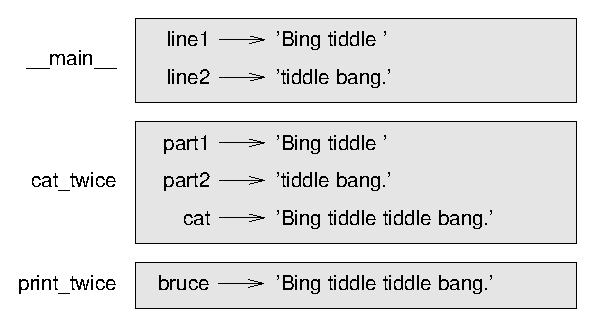
\includegraphics{figs/stack.eps}}
\afterfig

The frames are arranged in a stack that indicates which function
called which, and so on.  In this example, \verb"print_twice"
was called by \verb"cat_twice", and \verb"cat_twice" was called by 
\verb"__main__", which is a special name for the topmost frame.  When
you create a variable outside of any function, it belongs to 
\verb"__main__".

Each parameter refers to the same value as its corresponding
argument.  So, {\tt part1} has the same value as
{\tt line1}, {\tt part2} has the same value as {\tt line2},
and {\tt bruce} has the same value as {\tt cat}.

If an error occurs during a function call, Python prints the
name of the function, and the name of the function that called
it, and the name of the function that called {\em that}, all the
way back to \verb"__main__".

For example, if you try to access {\tt cat} from within 
\verb"print_twice", you get a {\tt NameError}:

\beforeverb
\begin{verbatim}
Traceback (innermost last):
  File "test.py", line 13, in __main__
    cat_twice(line1, line2)
  File "test.py", line 5, in cat_twice
    print_twice(cat)
  File "test.py", line 9, in print_twice
    print cat
NameError: name 'cat' is not defined
\end{verbatim}
\afterverb
%
This list of functions is called a {\bf traceback}.  It tells you what
program file the error occurred in, and what line, and what functions
were executing at the time.  It also shows the line of code that
caused the error.

\index{traceback}

The order of the functions in the traceback is the same as the
order of the frames in the stack diagram.  The function that is
currently running is at the bottom.


\section{Boolean functions}
\label{boolean}

\index{boolean function}

Functions can return booleans, which is often convenient for hiding
complicated tests inside functions.  For example:

\beforeverb
\begin{verbatim}
def is_divisible(x, y):
    if x % y == 0:
        return True
    else:
        return False
\end{verbatim}
\afterverb
%
It is common to give boolean functions names that sound like yes/no
questions; \verb"is_divisible" returns either {\tt True} or {\tt False}
to indicate whether {\tt x} is divisible by {\tt y}.

Here is an example:

\beforeverb
\begin{verbatim}
>>>   is_divisible(6, 4)
False
>>>   is_divisible(6, 3)
True
\end{verbatim}
\afterverb
%
The result of the {\tt ==} operator is a boolean, so we can write the
function more concisely by returning it directly:

\beforeverb
\begin{verbatim}
def is_divisible(x, y):
    return x % y == 0
\end{verbatim}
\afterverb
%
Boolean functions are often used in conditional statements:

\index{conditional statement}
\index{statement!conditional}

\beforeverb
\begin{verbatim}
if is_divisible(x, y):
    print 'x is divisible by y'
\end{verbatim}
\afterverb
%
It might be tempting to write something like:

\beforeverb
\begin{verbatim}
if is_divisible(x, y) == True:
    print 'x is divisible by y'
\end{verbatim}
\afterverb
%
But the extra comparison is unnecessary.

\begin{ex}
Write a function \verb"is_between(x, y, z)" that
returns {\tt True} if $x \le y \le z$ or {\tt False} otherwise.
\end{ex}

% TBD - May want to talk about "guarding" code here - lots removed

\section{Debugging}
\label{factdebug}

\index{debugging}

Breaking a large program into smaller functions creates natural
checkpoints for debugging.  If a function is not working, there are
three possibilities to consider:

\begin{itemize}

\item There is something wrong with the arguments the function
is getting; a precondition is violated.

\item There is something wrong with the function; a postcondition
is violated.

\item There is something wrong with the return value or the
way it is being used.

\end{itemize}

To rule out the first possibility, you can add a {\tt print} statement
at the beginning of the function and display the values of the
parameters (and maybe their types).  Or you can write code
that checks the preconditions explicitly.

\index{precondition}
\index{postcondition}

If the parameters look good, add a {\tt print} statement before each
{\tt return} statement that displays the return value.  If
possible, check the result by hand.  Consider calling the
function with values that make it easy to check the result
(as in Section~\ref{incremental development}).

If the function seems to be working, look at the function call
to make sure the return value is being used correctly (or used
at all!).

\index{flow of execution}

Adding print statements at the beginning and end of a function
can help make the flow of execution more visible.

If you are confused about the flow of execution, this kind of
output can be helpful.  It takes some time to develop effective
scaffolding, but a little bit of scaffolding can save a lot of debugging.


\section{Glossary}

\begin{description}

\item[temporary variable:]  A variable used to store an intermediate value in
a complex calculation.
\index{temporary variable}
\index{variable!temporary}

\item[dead code:]  Part of a program that can never be executed, often because
it appears after a {\tt return} statement.
\index{dead code}

\item[{\tt None}:]  A special value returned by functions that
have no return statement or a return statement without an argument.
\index{None special value}
\index{special value!None}

\item[local variable:]  A variable defined inside a function.  A local
variable can only be used inside its function.
\index{local variable}

\item[global variable:]  A variable defined outside a function.  Global
variables can be accessed from any function.
\index{global variable}

\item[declaration:] A statement like {\tt global} that tells the
interpreter something about a variable.
\index{declaration}


\item[incremental development:]  A program development plan intended to
avoid debugging by adding and testing only
a small amount of code at a time.
\index{incremental development}

\item[scaffolding:]  Code that is used during program development but is
not part of the final version.
\index{scaffolding}

\item[guardian:]  A programming pattern that uses a conditional
statement to check for and handle circumstances that
might cause an error.
\index{guardian pattern}
\index{pattern!guardian}

\item[stack diagram:]  A graphical representation of a stack of functions,
their variables, and the values they refer to.
\index{stack diagram}

\item[frame:]  A box in a stack diagram that represents a function call.
It contains the local variables and parameters of the function.
\index{function frame}
\index{frame}

\item[call graph:] A diagram that shows every frame created during
the execution of a program, with an arrow from each caller to
each callee. 

\index{call graph}
\index{diagram!call graph}

\item[traceback:]  A list of the functions that are executing,
printed when an exception occurs.
\index{traceback}

\item[flag:] A boolean variable used to indicate whether a condition
is true.
\index{flag}


\end{description}


\section{Exercises}

\begin{ex}
\index{stack diagram}

Draw a stack diagram for the following
program.  What does the program print?

\beforeverb
\begin{verbatim}
def b(z):
    prod = a(z, z)
    print z, prod
    return prod

def a(x, y):
    x = x + 1
    return x * y

def c(x, y, z):
    sum = x + y + z
    pow = b(sum)**2
    return pow

x = 1
y = x + 1
print c(x, y+3, x+y)
\end{verbatim}
\afterverb

\end{ex}



\begin{ex}
\label{palindrome}

\index{palindrome}

A palindrome is a word that is spelled the same backward and
forward, like ``noon'' and ``redivider''.  Recursively, a word
is a palindrome if the first and last letters are the same
and the middle is a palindrome.

The following are functions that take a string argument and
return the first, last, and middle letters:

\beforeverb
\begin{verbatim}
def first(word):
    return word[0]

def last(word):
    return word[-1]

def middle(word):
    return word[1:-1]
\end{verbatim}
\afterverb
%
We'll see how they work in Chapter~\ref{strings}.

\begin{enumerate}

\item Type these functions into a file named {\tt palindrome.py}
and test them out.  What happens if you call {\tt middle} with
a string with two letters?  One letter?  What about the empty
string, which is written \verb"''" and contains no letters?

\item Write a function called \verb"is_palindrome" that takes
a string argument and returns {\tt True} if it is a palindrome
and {\tt False} otherwise.  Remember that you can use the
built-in function {\tt len} to check the length of a string.

\end{enumerate}

\end{ex}

\begin{ex}
A number, $a$, is a power of $b$ if it is divisible by $b$
and $a/b$ is a power of $b$.  Write a function called
\verb"is_power" that takes parameters {\tt a} and {\tt b}
and returns {\tt True} if {\tt a} is a power of {\tt b}.
\end{ex}


\begin{ex}

\index{greatest common divisor (GCD)}
\index{GCD (greatest common divisor)}

The greatest common divisor (GCD) of $a$ and $b$ is the largest number
that divides both of them with no remainder\footnote{This exercise is
  based on an example from Abelson and Sussman's {\em Structure and
    Interpretation of Computer Programs}.}.

One way to find the GCD of two numbers is Euclid's algorithm,
which is based on the observation that if $r$ is the remainder
when $a$ is divided by $b$, then $gcd(a, b) = gcd(b, r)$.
As a base case, we can consider $gcd(a, 0) = a$.

\index{Euclid's algorithm}
\index{algorithm!Euclid}

Write a function called
\verb"gcd" that takes parameters {\tt a} and {\tt b}
and returns their greatest common divisor.  If you need
help, see \url{wikipedia.org/wiki/Euclidean_algorithm}.

\end{ex}





\chapter{Networked programs}

While many of the examples in this book have focused on reading
files and looking for data in those files, there are many different
sources of information when one considers the Internet.

In this chapter we will pretend to be a web browser and retrieve web
pages using the HyperText Transport Protocol (HTTP).  Then we will read
through the web page data and parse it.

\section{HyperText Transport Protocol - HTTP}

The network protocol that powers the web is actually quite simple and 
there is built-in support in Python called {\tt sockets} which makes it very 
easy to make network connections and retrieve data over those
sockets in a Python program.

A {\bf socket} is much like a file, except that it 
provides a two-way connection between two 
programs with a single socket.  
You can both read from and write to the same socket.  If you write somthing to 
a socket it is sent to the application at the other end of the socket.  If you 
read from the socket, you are given the data which the other application has sent.

But if you try to read a socket when the program on the other end of the socket
has not sent any data - you just sit and wait.  If the programs on both ends
of the socket simply wait for some data without sending anything, they will wait for
a very long time.

So an important part of programs that communicate over the Internet is to have some
sort of protocol.   A protocol is a set of precise rules that determine who
is to go first, what they are to do, and then what are the responses to that message,
and who sends next and so on.  In a sense the two applications at either end 
of the socket are doing a dance and making sure not to step on each other's toes.

There are many documents which describe these network protocols.  The HyperText Transport 
Protocol is described in the following document:

\url{http://www.w3.org/Protocols/rfc2616/rfc2616.txt}

This is a long and complex 176 page document with a lot of detail.  If you 
find it interesting feel free to read it all.  But if you take a look around page 36 of
RFC2616 you will find the syntax for the GET request.  If you read in detail, you will
find that to request a document from a web server, we make a connection to 
the {\tt www.py4inf.com} server on port 80, and then send a line of the form:

{\tt GET http://www.py4inf.com/code/romeo.txt HTTP/1.0 }

Where the second parameter is the web page we are requesting and then 
we also send a blank line.  The web server will respond with some 
header information about the document and a blank line
followed by the document content.

\section{The World's Simplest Web Browser}

Perhaps the easiest way to show how the HTTP protocol works is to write a very 
simple Python program that makes a connection to a web server and following
the rules of the HTTP protocol, requests a document 
and displays what the server sends back.

\beforeverb
\begin{verbatim}
import socket

mysock = socket.socket(socket.AF_INET, socket.SOCK_STREAM)
mysock.connect(("www.py4inf.com", 80))
mysock.send("GET http://www.py4inf.com/code/romeo.txt HTTP/1.0\n\n")

while True:
    data = mysock.recv(512)
    if ( len(data) < 1 ) :
        break
    print data

mysock.close()
\end{verbatim}
\afterverb
%
First the program makes a connection to port 80 on 
the server www.py4inf.com.
Since our program is playing the role of the "web browser" the HTTP
protocol says we must send the GET command followed by a blank line.

Once we send that blank line, we write a loop that receives data 
in 512 character chunks from the socket and prints the data out 
until there is no more data to read (i.e. the recv() returns 
an empty string).

The program produces the following output:

\beforeverb
\begin{verbatim}
HTTP/1.1 200 OK
Date: Sun, 14 Mar 2010 23:52:41 GMT
Server: Apache
Last-Modified: Tue, 29 Dec 2009 01:31:22 GMT
ETag: "143c1b33-a7-4b395bea"
Accept-Ranges: bytes
Content-Length: 167
Connection: close
Content-Type: text/plain

But soft what light through yonder window breaks
It is the east and Juliet is the sun
Arise fair sun and kill the envious moon
Who is already sick and pale with grief
\end{verbatim}
\afterverb
%
The output starts with headers which the web server sends
to describe the document.
For example, the {\tt Content-Type } header indicated that
the document is a plain text document ({\tt text/plain}).

After the server sends us the headers, it adds a blank line
to indicate the end of the headers and then sends the actual
data of the file {\tt romeo.txt}.

This example shows how to make a low-level network connection
with sockets.   Sockets can be use to communicate with a web
server or with a mail server or many other kinds of servers.
All that is needed is to find the document which describes
the protocol and write the code to send and receive the data
according to the protocol.

However, since the protocol that we use most commonly is
the HTTP (i.e. the web) protocol, Python has a special 
library specifically designed to support the HTTP protocol 
for the retrieval of
documents and data over the web.

\section{Retrieving web pages with {\tt urllib}}

The {\tt urllib} library makes it very easy to retrieve
web pages and process the data in Python.   Using {\tt urllib}
you can treat a web page much like a file.   You simply
indicate which web page you would like to retrieve and
{\tt urllib} handles all of the HTTP protocol details.

The equivalent code to read the {\tt romeo.txt} file
from the web using {\tt urllib} is as follows:

\beforeverb
\begin{verbatim}
import urllib

fhand = urllib.urlopen('http://www.py4inf.com/code/romeo.txt')
for line in fhand:
   print line.strip()
\end{verbatim}
\afterverb
%
Once the web page has been opened with 
{\tt urllib.urlopen} we can treat it like 
a file and read through it using a 
{\tt for} loop.   

When the program runs, we only see the output
of the contents of the file.   The headers
are still sent, but the {\tt urllib} code
consumes the headers and only returns the 
data to us.

\beforeverb
\begin{verbatim}
But soft what light through yonder window breaks
It is the east and Juliet is the sun
Arise fair sun and kill the envious moon
Who is already sick and pale with grief
\end{verbatim}
\afterverb
%

As an example, we can write 
a program to retrieve the data for
{\tt romeo.txt} and compute the frequency
of each word in the file as follows:

\beforeverb
\begin{verbatim}
import urllib

counts = dict()
fhand = urllib.urlopen('http://www.py4inf.com/code/romeo.txt')
for line in fhand:
   words = line.split()
   for word in words:
      counts[word] = counts.get(word,0) + 1   
print counts
\end{verbatim}
\afterverb
%
Again, once we have opened the web page, 
we can read it like a local file.

\section{Parsing HTML and scraping the web}

One of the common uses of the {\tt urllib} capability in Python is 
to {\bf scrape} the web.   Web scraping is when we write a program
that pretends to be a web browser and retrieves pages and then 
examines the data in those pages looking for patterns.

As an example, a search engine such as Google will look at the source 
of one web page and extract the links to other pages and retrieve
those pages, extracting links, and so on.   Using this technique,
Google {\bf spiders} its way through nearly all of the pages on 
the web.   
Google also uses the frequency of links from pages it finds 
to a particular page as one measure of how ``important'' 
a page is and how highly the page should appear in its search results.

There are a number of Python libraries which can help you parse
HTML and extract data from the pages.  Each of the libraries
has its strengths and weaknesses and you can pick one based on 
your needs.

As an example, we will simply parse some HTML input 
and extract links using Python string functions.   Here is a 
simple web page:

\beforeverb
\begin{verbatim}
<h1>The First Page</h1>
<p>
If you like, you can switch to the
<a href="http://www.dr-chuck.com/page2.htm">
Second Page</a>.
</p>
\end{verbatim}
\afterverb
%
We will read through the page and key off the ``href'' string
in the line.   We will then use simple string manipulation
to  extract the information between the double quotes as follows:

\beforeverb
\begin{verbatim}
import urllib

url = raw_input('Enter - ')
fhand = urllib.urlopen(url)
for line in fhand:
   pos = line.find('href="')
   if pos < 1 : continue
   rest = line[pos+6:]
   end = rest.find('"')
   if end < 1 : continue
   link = rest[:end]
   print link
\end{verbatim}
\afterverb
%
The program prompts for a web address, then opens the web
address and starts looping through the lines of the web page.
First it looks for lines with ``href'' and skips the lines
that do not have the ``href'' string.  On lines with the 
``href'' string, the code skips past the ``href'', equals sign, 
and double quote and takes the rest of the line.

It then searches for the next double quote in the rest of the 
line and treats the link as the text up to but not 
including the second double quote.

When the program is run it looks as follows:

\beforeverb
\begin{verbatim}
python urllinks.py 
Enter - http://www.dr-chuck.com/page1.htm
http://www.dr-chuck.com/page2.htm

python urllinks.py 
Enter - http://www.py4inf.com/
/glike.css
py4inf_cover.jpg
http://www.greenteapress.com/thinkpython/thinkpython.html
http://allendowney.com/
http://www.si502.com/
http://www.lib.umich.edu/espresso-book-machine
http://www.py4inf.com/code
http://www.pythonlearn.com/
\end{verbatim}
\afterverb
%
\section{Glossary}

\begin{description}

\item[port:] A number that generally indicates which application 
you are contacting when you make a socket connection to a server.
As an example, web traffic usually uses port 80 while e-mail 
traffic uses port 50.
\index{port}

\item[scrape:] When a program pretends to be a web browser and
retrieves a web page and then looks at the web page content. 
Often programs are following the links in one page to find the next
page so they can traverse a network of pages or a social network.
\index{socket}

\item[socket:] A network connection between two applications
where the applications can send and receive data in either direction.
\index{socket}

\item[spider:] The act of a web search engine retrieving a page and
then all the pages linked from a page and so on until they have 
nearly all of the pages on the Internet which they 
use to build their search index.
\index{spider}

\end{description}

\section{Exercises}

\begin{ex}
Download the Google Application Engine Python SDK from 

\url{http://code.google.com/appengine/downloads.html}

And create the ``hello world'' application in Google App Engine
and get it up and running
on your computer.  Then adapt the simple {\tt socket} program to 
connect to your web server running at {\tt http://localhost:8080/}
instead of {\tt http://www.py4inf.com/code/romeo.txt}.  Remember that
the ``8080'' is the non-default HTTP port number while 80 is the 
default http port number.

The output should look as follows:
\beforeverb
\begin{verbatim}
HTTP/1.0 200 Good to go

Server: Development/1.0
Date: Wed, 17 Mar 2010 20:30:59 GMT
Content-Type: text/plain
Cache-Control: no-cache
Expires: Fri, 01 Jan 1990 00:00:00 GMT
Content-Length: 17

Hello there Chuck
\end{verbatim}
\afterverb
%
\end{ex}

\begin{ex}
Change the program which uses {\tt urllib} and reads and prints
the data to talk to your web server running at 
{\tt http://localhost:8080/}.
How is the output different from the previous exercise and why?
\end{ex}


\chapter{Using Web Services}

Once it became easy to retrieve documents and parse documents 
over HTTP using programs, it did not take long to develop 
an approach where we started producing documents that were specifically
designed to be consumed by other 
programs (i.e. not HTML to be displayed in a browser).

The most common approach when two programs are exchanging data across 
the web is to exchange the data in a format called the ``eXtensible Markup 
Language'' or XML.  

\section{eXtensible Markup Language - XML}

XML looks very similar to HTML, but XML is more structured 
than HTML.  Here is a sample of an XML document:

\beforeverb
\begin{verbatim}
<person>
  <name>Chuck</name>
  <phone type="intl">
     +1 734 303 4456
   </phone>
   <email hide="yes"/>
</person>
\end{verbatim}
\afterverb
%
\section{Parsing XML}

Here is a simple application that parses some XML
and extracts some data elements from the XML:

\index{ElementTree}
\index{ElementTree!fromstring}
\index{ElementTree!find}
\beforeverb
\begin{verbatim}
import xml.etree.ElementTree as ET

data = '''
<person>
  <name>Chuck</name>
  <phone type="intl">
     +1 734 303 4456
   </phone>
   <email hide="yes"/>
</person>'''

tree = ET.fromstring(data)
print 'Name:',tree.find('name').text
print 'Attr:',tree.find('email').get('hide')
\end{verbatim}
\afterverb
%
Calling {\tt fromstring} converts the string representation
of the XML into a 'tree' of XML nodes.  When the
XML is in a tree, we have a series of methods which we can call to 
extract portions of data from the XML.  

The {\tt find} function searches through the 
XML tree and retrieves a {\bf node} that matches the specified tag.
Each node can have some text, some attributes (i.e. like hide) and
some ``child'' nodes.   Each node can be the top of a tree of nodes.

\beforeverb
\begin{verbatim}
Name: Chuck
Attr: yes
\end{verbatim}
\afterverb
%
Using an XML parser such as {\tt ElementTree} has the advantage
that while the XML in this example is quite simple, it turns
out that there are many rules regarding valid XML and using 
{\tt ElementTree} allows us to extract data from XML without 
worrying about the rules of XML syntax.

\section{Looping through nodes}

Often the XML has multiple nodes and we need to write a loop
to process all of the nodes.  In the following program, 
we loop through all of the {\tt user} nodes:

\index{ElementTree!findall}
\index{ElementTree!get}
\beforeverb
\begin{verbatim}
import xml.etree.ElementTree as ET

input = '''
<stuff>
    <users>
        <user x="2">
            <id>001</id>
            <name>Chuck</name>
        </user>
        <user x="7">
            <id>009</id>
            <name>Brent</name>
            </user>
        </users>
</stuff>'''

stuff = ET.fromstring(input)
lst = stuff.findall("users/user")
print 'User count:', len(lst)

for item in lst:
    print 'Name', item.find('name').text
    print 'Id', item.find('id').text
    print 'Attribute', item.get("x")
\end{verbatim}
\afterverb
%
The {\tt findall} method retrieves a Python list of sub-trees that
represent the {\tt user} structures in the XML tree.  Then we can 
write a {\tt for} loop that looks at each of the user nodes, and 
prints the {\tt name} and {\tt id} text elements as well as the 
{\tt x} attribute from the {\tt user} node.

\beforeverb
\begin{verbatim}
User count: 2
Name Chuck
Id 001
Attribute 2
Name Brent
Id 009
Attribute 7
\end{verbatim}
\afterverb
%

\section{Application Programming Interfaces (API)}

We now have the ability to exchange data between applications using HyperText
Transport Protocol (HTTP) and a way to represent complex data that we are 
sending back and forth between these applications using eXtensible 
Markup Language (XML).

The next step is to begin to define and document ``contracts'' between 
applications using these techniques. The general name for these 
application-to-application contracts is {\bf Application Program 
Interfaces} or APIs.  When we use an API, generally one program
makes a set of {\bf services} available for use by other applications
and publishes the APIs (i.e. the ``rules'') which must be followed to 
access the services provided by the program.

When we begin to build our programs where the functionality of
our program includes access to services provided by other programs, 
we call the approach a {\bf Service-Oriented Architecture} or SOA.
A SOA approach is one where our overall application makes use of 
the services of other applications.  A non-SOA approach is where the
application is a single stand-alone application which contains all of the
code necessary to implement the application.

We see many examples of SOA when we use the web.  We can go to a single 
web site and book air travel, hotels, and automobiles all from a 
single site.  The data for hotels is not stored on the airline computers. 
Instead, the airline computers contact the services on the hotel computers
and retrieve the hotel data and present it to the user.  When the user
agrees to make a hotel reservation using the airline site, the airline site uses
another web service on the hotel systems to actually make the reservation.
And when it comes to charge your credit card for the whole transaction, 
still other computers become involved in the process.

A Service-Oriented Architecture has many advantages including: (1) we 
always maintain only one copy of data - this is particularly important
for things like hotel reservations where we do not want to over-commit
and (2) the owners of the data can set the rules about the use of their 
data.   With these advantages, a SOA system must be carefully designed
to have good performance and meet the user's needs.

When an application makes a set of services in its API available over the web, 
we call these {\bf web services}. 

\section{Twitter web services}

You are probably familiar with the Twitter web site and its
applications \url{http://www.twitter.com}.  Twitter has a very unique
approach to its API/web services in that all of its data is available
to non-Twitter applications using the Twitter API.

Because Twitter has been so liberal in allowing access to its data,
it has enabled thousands of software developers to build their own
customized Twitter-based software.  These additional applications greatly
increase the value of Twitter far beyond simply a web site.  The 
Twitter web services allow the building of whole new applications that
the Twitter team may never have thought of.  It is said that over 90 percent
of the use of Twitter is through the API (i.e. not through the {\tt twitter.com}
web user interface).

You can view the Twitter API documentation at 
\url{http://apiwiki.twitter.com/}.  The Twitter API is an example
of the REST style of web services.
We will focus on the Twitter API
to retrieve a list of a user's friends and their statuses.  As an 
example, you can visit the following URL:

\url{http://api.twitter.com/1/statuses/friends/drchuck.xml}

To see a list of the friends of the twitter account {\tt drchuck}.
It may look like a mess in your browser.   To see the actual XML
returned by Twitter, you can view the source of the returned
``web page''.

We can retrieve this same XML using Python using the {\tt urllib}
utility:

\beforeverb
\begin{verbatim}
import urllib

TWITTER_URL = 'http://api.twitter.com/l/statuses/friends/ACCT.xml'

while True:
    print ''
    acct = raw_input('Enter Twitter Account:')
    if ( len(acct) < 1 ) : break
    url = TWITTER_URL.replace('ACCT', acct)
    print 'Retrieving', url
    document = urllib.urlopen (url).read()
    print document[:250]
\end{verbatim}
\afterverb
%
The program prompts for a Twitter account and opens the URL
for the friends and statuses API and then retrieves the 
text from the URL and shows us the first 250 characters of
the text.

\beforeverb
\begin{verbatim}
python twitter1.py

Enter Twitter Account:drchuck
Retrieving http://api.twitter.com/l/statuses/friends/drchuck.xml
<?xml version="1.0" encoding="UTF-8"?>
<users type="array">
<user>
  <id>115636613</id>
  <name>Steve Coppin</name>
  <screen_name>steve_coppin</screen_name>
  <location>Kent, UK</location>
  <description>Software developing, best practicing, agile e

Enter Twitter Account:
\end{verbatim}
\afterverb
%
In this application, we have retrieved the XML exactly as if it were
an HTML web page.  If we wanted to extract data from the XML, we 
could use Python string functions but this would become pretty complex
as we tried to really start to dig into the XML in detail.

If we were to dump out some of the retrieved XML it would look roughly as follows:

\beforeverb
\begin{verbatim}
<?xml version="1.0" encoding="UTF-8"?>
<users type="array">
  <user>
    <id>115636613</id>
    <name>Steve Coppin</name>
    <screen_name>steve_coppin</screen_name>
    <location>Kent, UK</location>
    <status>
      <id>10174607039</id>
      <source>web</source>
      </status>
  </user>
  <user>
    <id>17428929</id>
    <name>davidkocher</name>
    <screen_name>davidkocher</screen_name>
    <location>Bern</location>
    <status>
      <id>10306231257</id>
      <text>@MikeGrace If possible please post a detailed bug report </text>
    </status>
  </user>
  ...
\end{verbatim}
\afterverb
%
The top level tag is a {\tt users} and there are multiple {\tt user} tags
below within the {\tt users} tag.   There is also a {\tt status} tag below
the {\tt user} tag.  

\section{Handling XML data from an API}

When we receive well-formed XML data from an API, we generally use
an XML parser such as {\tt ElementTree} to extract information from
the XML data.

In the program below, we retrieve the friends and statuses from
the Twitter API and then parse the returned XML to show the first
four friends and their statuses.

\beforeverb
\begin{verbatim}
import urllib
import xml.etree.ElementTree as ET

TWITTER_URL = 'http://api.twitter.com/l/statuses/friends/ACCT.xml'

while True:
    print ''
    acct = raw_input('Enter Twitter Account:')
    if ( len(acct) < 1 ) : break
    url = TWITTER_URL.replace('ACCT', acct)
    print 'Retrieving', url
    document = urllib.urlopen (url).read()
    print 'Retrieved', len(document), 'characters.' 
    tree = ET.fromstring(document)
    count = 0
    for user in tree.findall('user'):
        count = count + 1
        if count > 4 : break
        print user.find('screen_name').text
        status =  user.find('status')
        if status : 
            txt = status.find('text').text
            print '  ',txt[:50]
\end{verbatim}
\afterverb
%
We use the {\tt findall} method to get a list of the {\tt user} 
nodes and loop through the list using a {\tt for } loop.  
For each {\tt user} node, we pull out the text of the \verb"screen_name" node
and then pull out the {\tt status} node.   If there is a {\tt status}
node, we pull out the text of the {\tt text} node and print the first 50 
characters of the status text.

The pattern is pretty straightforward, we use {\tt findall} and {\tt find}
to pull out a list of nodes or a single node and then if a node is a complex
element with more sub-nodes we look deeper into the node until we reach the 
text element that we are interested in.

The program runs as follows:

\beforeverb
\begin{verbatim}
python twitter2.py 

Enter Twitter Account:drchuck
Retrieving http://api.twitter.com/l/statuses/friends/drchuck.xml
Retrieved 193310 characters.
steve_coppin
   Looking forward to some "oh no the markets closed,
davidkocher
   @MikeGrace If possible please post a detailed bug 
hrheingold
   From today's Columbia Journalism Review, on crap d
huge_idea
   @drchuck  #cnx2010 misses you, too.  Thanks for co

Enter Twitter Account:hrheingold
Retrieving http://api.twitter.com/l/statuses/friends/hrheingold.xml
Retrieved 208081 characters.
carr2n
   RT @tysone: Saturday's proclaimation by @carr2n pr
tiffanyshlain
   RT @ScottKirsner: Turning smartphones into a tool 
soniasimone
   @ACCompanyC Funny, smart, cute, and also nice! He 
JenStone7617
   Watching "Changing The Equation: High Tech Answers

Enter Twitter Account:
\end{verbatim}
\afterverb
%
While the code for parsing the XML and extracting the fields
using {\tt ElementTree} takes a few lines to express what 
we are looking for in the XML, it is much simpler than trying 
to use Python string parsing to pull apart the XML and find 
the data elements.

\section{Glossary}

\begin{description}

\item[API:] Application Program Interface - A contract between
applications that defines the patterns of interaction between 
two application components.
\index{API}

\item[ElementTree:] A built-in Python library used to parse XML data.
\index{ElementTree}

\item[REST:] REpresentational State Transfer - A style of Web Services 
that provide access to resources within an application using the HTTP
protocol.
\index{ElementTree}

\item[SOA:] Service Oriented Architecture - when an application is 
made of components connected across a network.
\index{SOA}
\index{Service Oriented Architecture}

\item[XML:] eXtensible Markup Language - A format that allows for 
the markup of structured data.
\index{XML}
\index{eXtensible Markup Language}

\end{description}

\section{Exercises}

\begin{ex}
Change the program that retrieves twitter data to also
print out the location for each of the friends
indented under the name by two spaces as follows:

\beforeverb
\begin{verbatim}
Enter Twitter Account:drchuck
Retrieving http://api.twitter.com/l/statuses/friends/drchuck.xml
Retrieved 194533 characters.
steve_coppin
   Kent, UK
   Looking forward to some "oh no the markets closed,
davidkocher
   Bern
   @MikeGrace If possible please post a detailed bug 
hrheingold
   San Francisco Bay Area
   RT @barrywellman: Lovely AmBerhSci Internet & Comm
huge_idea
   Boston, MA
   @drchuck  #cnx2010 misses you, too.  Thanks for co
\end{verbatim}
\afterverb
%
\end{ex}

\chapter{Regular expressions}

\section{More accurate searching}

\section{Building regular expressions}

\section{Applications of regular expressions}

\section{Regular expressions at the command line (Advanced)}


\chapter{Automating common tasks}

One of the great advantages of the Python language is the ability
to write programs that scan through your computer and 
perform some operation on each file.  
Files are organized into {\bf directories} (also called ``folders'').
Simple Python scripts
can make short work of simple tasks that must be done to 
hundreds or thousands of files
spread across a directory tree.

To walk through all the directories and files in a tree we use 
{\tt os.walk} and a {\tt for} loop.  This is similar to how 
{\tt open} allows us to write a loop to read the contents of a file,
{\tt socket} allows us to write a loop to read the contents of a network connection, and
{\tt urllib} allows us to open a web document and loop through its contents.

\section{Filenames and paths}
\label{paths}

\index{filename}
\index{path}
\index{directory}
\index{folder}

Every running program has a ``current directory,'' which is the
default directory for most operations.  
For example, when you open a file for reading, Python looks for it in the
current directory.

\index{os module}
\index{module!os}

The {\tt os} module provides functions for working with files and
directories (``os'' stands for ``operating system'').  {\tt os.getcwd}
returns the name of the current directory:

\index{getcwd function}
\index{function!getcwd}

\beforeverb
\begin{verbatim}
>>> import os
>>> cwd = os.getcwd()
>>> print cwd
/home/dinsdale
\end{verbatim}
\afterverb
%
{\tt cwd} stands for {\bf current working directory}.  The result in
this example is {\tt /home/dinsdale}, which is the home directory of a
user named {\tt dinsdale}.

\index{working directory}
\index{directory!working}

A string like {\tt cwd} that identifies a file is called a {\bf path}.
A {\bf relative path} starts from the current directory;
an {\bf absolute path} starts from the topmost directory in the
file system.

\index{relative path}
\index{path!relative}
\index{absolute path}
\index{path!absolute}

The paths we have seen so far are simple filenames, so they are
relative to the current directory.  To find the absolute path to
a file, you can use {\tt os.path.abspath}:

\beforeverb
\begin{verbatim}
>>> os.path.abspath('memo.txt')
'/home/dinsdale/memo.txt'
\end{verbatim}
\afterverb
%
{\tt os.path.exists} checks
whether a file or directory exists:

\index{exists function}
\index{function!exists}

\beforeverb
\begin{verbatim}
>>> os.path.exists('memo.txt')
True
\end{verbatim}
\afterverb
%
If it exists, {\tt os.path.isdir} checks whether it's a directory:

\beforeverb
\begin{verbatim}
>>> os.path.isdir('memo.txt')
False
>>> os.path.isdir('music')
True
\end{verbatim}
\afterverb
%
Similarly, {\tt os.path.isfile} checks whether it's a file.

{\tt os.listdir} returns a list of the files (and other directories)
in the given directory:

\beforeverb
\begin{verbatim}
>>> os.listdir(cwd)
['music', 'photos', 'memo.txt']
\end{verbatim}
\afterverb
%


\section{Example: Cleaning up a photo directory}

I will start with a simple real example problem and then walk through 
the solution in a series of simple Python scripts.  I had built a 
bit of Flickr-like software that stored my cell-phone photos on a server
when I would send the photos to the server using E-Mail or MMS.  I wrote
this before Flickr existed and kept using it after Flickr existed because
I wanted to keep original copies of my images forever.

I would also send a simple one-line text description in the MMS message
or the subject line of the E-Mail message.  I stored these messages
in a text file in the same directory as the image file.   I had come up 
with a directory structure based on the month, year, day and time the 
photo was taken.   The following would be an example of the naming for 
one photo and its existing description:

\beforeverb
\begin{verbatim}
./2006/03/24-03-06_2018002.jpg
./2006/03/24-03-06_2018002.txt
\end{verbatim}
\afterverb
%
After seven years, I had a lot of photos and captions.  But over the years
as I switched cell phones, sometimes my code to pull out the caption would
break and add a bunch of useless data from the message instead of a caption.  

So I wanted to go through these files and figure out which of the 
text files were really captions and which were junk and then delete the bad
files.  The first thing to do was to get a simple inventory of 
how many text files I had all in all of the sub-folders
using the following program:

\beforeverb
\begin{verbatim}
import os
count = 0
for (dirname, dirs, files) in os.walk('.'):
   for filename in files:
       if filename.endswith('.txt') :
           count = count + 1
print 'Files:', count

python txtcount.py
Files: 1917
\end{verbatim}
\afterverb
%
The key bit of code that makes this possible is the {\tt os.walk}
library in Python.  When we call {\tt os.walk} and give it a starting
directory, it will ``walk'' through all of the directories 
and subdirectories recursively.   The string ``.'' indicates
to start in the current directory and walk downward.
As it encounters each directory,
we get three values in a tuple in the body of the {\tt for} loop.  
The first value is the curent
directory name, the second value is the list of sub-directories 
in the current directory, and the third value is a list of files
in the current directory.

We do not have to explicitly look into each of the sub-directories
because we can count on {\tt os.walk} to visit every 
folder eventually.  But we do want to look at each file so 
we write a simple {\tt for} loop to examine each of the files 
in the current directory.   We check each file to see if 
it ends with ``.txt'' and then count the number of 
files through the whole directory tree that end with the
suffix ``.txt''.

Once we have a sense of how many files that end with ``.txt'', the next
thing to do is try to automatically
determine in Python which files are bad and which files
are good.   So we write a simple program to print out the
files and the size of each file:

\beforeverb
\begin{verbatim}
import os
from os.path import join
for (dirname, dirs, files) in os.walk('.'):
   for filename in files:
       if filename.endswith('.txt') :
           thefile = os.path.join(dirname,filename)
           print os.path.getsize(thefile), thefile
\end{verbatim}
\afterverb
%
Now instead of just counting the files, we create 
a file name by concatening the directory name with
the name of the file within the directory using
{\tt os.path.join}.   It is important to use 
{\tt os.path.join} instead of string concatenation 
because on Windows we use a backslash
(\verb"\") to construct file paths and on Linux
or Apple we use a forward slash (\verb"/") 
to construct file paths.  The {\tt os.path.join}
knows these differences and knows what system
we are running on and it does the proper concatenation
depending on the system.  So the same Python code
runs on either Windows or UNIX-style systems.

Once we have the full file name with directory
path, we use the {\tt os.path.getsize} utility
to get the size and print it out, producing the 
following output:

\beforeverb
\begin{verbatim}
python txtsize.py
...
18 ./2006/03/24-03-06_2303002.txt
22 ./2006/03/25-03-06_1340001.txt
22 ./2006/03/25-03-06_2034001.txt
...
2565 ./2005/09/28-09-05_1043004.txt
2565 ./2005/09/28-09-05_1141002.txt
...
2578 ./2006/03/27-03-06_1618001.txt
2578 ./2006/03/28-03-06_2109001.txt
2578 ./2006/03/29-03-06_1355001.txt
...
\end{verbatim}
\afterverb
%
Scanning the output, we notice that some files are pretty short and 
a lot of the files are pretty large and the same size (2578 and 2565). 
When we take a look at a few of these larger files by hand, 
it looks like the large 
files are nothing but a generic bit of identical HTML that came 
in from mail sent to my system from my T-Mobile phone:

\beforeverb
\begin{verbatim}
<html>
        <head>
                <title>T-Mobile</title>
...
\end{verbatim}
\afterverb
%
Skimming through the file, it looks like there is no good information
in these files so we can probably delete them.

But before we delete the files, lets write a program to look for files
that are more than one line long and show the contents of the file.
But lets not bother showing ourselves those files that are exactly
2578 or 2565 characters long since we know that these files have no useful
information.

So we write the following program:
\beforeverb
\begin{verbatim}
import os
from os.path import join
for (dirname, dirs, files) in os.walk('.'):
   for filename in files:
       if filename.endswith('.txt') :
           thefile = os.path.join(dirname,filename)
           size = os.path.getsize(thefile)
           if size == 2578 or size == 2565:
               continue
           fhand = open(thefile,"r")
           lines = list()
           for line in fhand:
               lines.append(line)
           fhand.close()
           if len(lines) > 1:
                print len(lines), thefile
                print lines[:4]
\end{verbatim}
\afterverb
%
We use a {\tt continue} to skip files with the two 
``bad sizes'' and then open the rest of the files
and read the lines of the file into a Python list
and if the file has more than one line we print
out how many lines are in the file and print out
the first three lines.

It looks like filtering out those two bad file sizes, and assuming
that all one line files are OK, we are down to some pretty clean
data:

\beforeverb
\begin{verbatim}
python txtcheck.py 
3 ./2004/03/22-03-04_2015.txt
['Little horse rider\r\n', '\r\n', '\r']
2 ./2004/11/30-11-04_1834001.txt
['Testing 123.\n', '\n']
3 ./2007/09/15-09-07_074202_03.txt
['\r\n', '\r\n', 'Sent from my iPhone\r\n']
3 ./2007/09/19-09-07_124857_01.txt
['\r\n', '\r\n', 'Sent from my iPhone\r\n']
3 ./2007/09/20-09-07_115617_01.txt
...
\end{verbatim}
\afterverb
%
But there is one more annoying pattern of files, 
there are some three-line files that consist of
two blank lines followed by a line that says
``Sent from my iPhone'' that have slipped 
into my data.   So we make the following change
to the program to deal with these files as well.

\beforeverb
\begin{verbatim}
           lines = list()
           for line in fhand:
               lines.append(line)
           if len(lines) == 3 and lines[2].startswith('Sent from my iPhone') :
               continue
           if len(lines) > 1:
                print len(lines), thefile
                print lines[:4]
\end{verbatim}
\afterverb
%
We simply check if we have a three line file and if the third 
line starts with the specified text, we skip it.

Now when we run the program, we only see four remaining 
multi-line files and all of those files look pretty reasonable:
\beforeverb
\begin{verbatim}
python txtcheck2.py 
3 ./2004/03/22-03-04_2015.txt
['Little horse rider\r\n', '\r\n', '\r']
2 ./2004/11/30-11-04_1834001.txt
['Testing 123.\n', '\n']
2 ./2006/03/17-03-06_1806001.txt
['On the road again...\r\n', '\r\n']
2 ./2006/03/24-03-06_1740001.txt
['On the road again...\r\n', '\r\n']
\end{verbatim}
\afterverb
%
If you look at the overall pattern of this program,
we have successively refined how we accept or reject
files and once we found a pattern that was 'bad' we used
{\tt continue} to skip the bad files so we could refine
our code to find more file patterns that were bad.

Now we are getting ready to delete the files and so 
we are going to flip the logic and instead of printing out 
the ``remaining good files'', we will print out the ``bad''
files that we are about to delete.
\beforeverb
\begin{verbatim}
import os
from os.path import join
for (dirname, dirs, files) in os.walk('.'):
   for filename in files:
       if filename.endswith('.txt') :
           thefile = os.path.join(dirname,filename)
           size = os.path.getsize(thefile)
           if size == 2578 or size == 2565:
               print 'T-Mobile:',thefile
               continue
           fhand = open(thefile,"r")
           lines = list()
           for line in fhand:
               lines.append(line)
           fhand.close()
           if len(lines) == 3 and lines[2].startswith('Sent from my iPhone') :
               print 'iPhone:', thefile
               continue
\end{verbatim}
\afterverb
%
So we can now see a list of candidate files that we are about
to delete and why these files are up for deleting.
The program produces the following output:
\beforeverb
\begin{verbatim}
python txtcheck3.py
...
T-Mobile: ./2006/05/31-05-06_1540001.txt
T-Mobile: ./2006/05/31-05-06_1648001.txt
iPhone: ./2007/09/15-09-07_074202_03.txt
iPhone: ./2007/09/15-09-07_144641_01.txt
iPhone: ./2007/09/19-09-07_124857_01.txt
...
\end{verbatim}
\afterverb
%
We can spot-check these files to make sure that we did not inadvertently
end up introducing a bug in our program or perhaps our logic 
caught some files we did not want to catch.

Once we are satisfied that this is the list of files we want to delete,
we make the following change to the program:
\beforeverb
\begin{verbatim}
           if size == 2578 or size == 2565:
               print 'T-Mobile:',thefile
               os.remove(thefile)
               continue
...
           if len(lines) == 3 and lines[2].startswith('Sent from my iPhone') :
               print 'iPhone:', thefile
               os.remove(thefile)
               continue
\end{verbatim}
\afterverb
%
In this version of the program, we will both print the file out 
and remove the bad files
using {\tt os.remove}.

\beforeverb
\begin{verbatim}
python txtdelete.py 
T-Mobile: ./2005/01/02-01-05_1356001.txt
T-Mobile: ./2005/01/02-01-05_1858001.txt
...
\end{verbatim}
\afterverb
%
Just for fun, run the program a second time and it will produce no output
since the bad files are already gone.

If we rerun {\tt txtcount.py} we can see that we have removed
899 bad files:
\beforeverb
\begin{verbatim}
python txtcount.py 
Files: 1018
\end{verbatim}
\afterverb
%
In this section, we have followed a sequence where we use Python 
to first look through directories and files looking for 
patterns.  We slowly use Python to help determine what we 
want to do to clean up our directories.  Once we
figure out which files are good and which files are 
not useful, we use Python to delete the files and 
perform the cleanup.

The problem you may need to solve can either be quite simple 
and might only depend on looking at the names of files,
or perhaps you need to read every single file and
look for patterns within the files.  Sometimes 
you will need to read all the files and make a change 
to some or of the files.  All of these are pretty 
straighforward once you understand how {\tt os.walk}
and the other {\tt os} utilities can be used.

\section{Pipes}

\index{shell}
\index{pipe}

Most operating systems provide a command-line interface,
also known as a {\bf shell}.  Shells usually provide commands
to navigate the file system and launch applications.  For
example, in Unix, you can change directories with {\tt cd},
display the contents of a directory with {\tt ls}, and launch
a web browser by typing (for example) {\tt firefox}.

\index{ls (Unix command)}
\index{Unix command!ls}

Any program that you can launch from the shell can also be
launched from Python using a {\bf pipe}.  A pipe is an object
that represents a running process.

For example, the Unix command\footnote{When using pipes to talk 
to operating system commands like {\tt ls}, it is important 
for you to know which operating system you are using and only
open pipes to commands that are supported on your operating system.}
{\tt ls -l} normally displays the
contents of the current directory (in long format).  You can
launch {\tt ls} with {\tt os.popen}:

\index{popen function}
\index{function!popen}

\beforeverb
\begin{verbatim}
>>> cmd = 'ls -l'
>>> fp = os.popen(cmd)
\end{verbatim}
\afterverb
%
The argument is a string that contains a shell command.  The
return value is a file pointer that behaves just like an open
file.  You can read the output from the {\tt ls} process one
line at a time with {\tt readline} or get the whole thing at
once with {\tt read}:

\index{readline method}
\index{method!readline}
\index{read method}
\index{method!read}

\beforeverb
\begin{verbatim}
>>> res = fp.read()
\end{verbatim}
\afterverb
%
When you are done, you close the pipe like a file:

\index{close method}
\index{method!close}

\beforeverb
\begin{verbatim}
>>> stat = fp.close()
>>> print stat
None
\end{verbatim}
\afterverb
%
The return value is the final status of the {\tt ls} process;
{\tt None} means that it ended normally (with no errors).

\section{Glossary}

\begin{description}

\item[absolute path:] A string that describes where a file or
directory is stored that starts at the ``top of the tree of directories''
so that it can be used to access the file or directory regardless
of the current working directory.
\index{path!absolute}

\item[checksum:] See also {\bf hashing}.  The term ``checksum'' 
comes from the need to verify if data was garbled as it was 
sent across a network or written to a backup medium and then
read back in.  When the data is written or sent, the sending system
computes a checksum and also sends the checksum.  When the 
data is read or received, the receiving system recomputes
the checksum from the received data and compares it to the 
received checksum.  If the checksums do not match, we must
assume that the data was garbled as it was transferred.
\index{checksum}

\item[current working directory:] The current directory that you 
are ``in''.  You can change your working directory using the 
{\tt cd} command on most systems in their command-line interfaces.
When you open a file in Python using just the file name with no path 
information the file must be in the current working directory
where you are runnig the program.
\index{directory!current}
\index{directory!working}
\index{directory!cwd}

\item[hashing:] Reading through a potentially large amount of data
and producing a unique checksum for the data.  The best hash functions
produce very few ``collisions'' where you can give two different
streams of data to the hash function and get back the same hash. 
MD5, SHA1, and SHA256 are examples of commonly used hash functions.
\index{hashing}

\item[pipe:] A pipe is a connection to a running program.  Using
a pipe, you can write a program to send data to another program
or receive data from that program.  A pipe is similar to a 
{\bf socket} except that a pipe only can be used to 
connect programs running on the same computer (i.e. not
across a network).
\index{pipe}

\item[relative path:] A string that describes where a file or
directory is stored {\emph relative} to the current working 
directory.
\index{path!relative}

\item[shell:] A command-line interface to an operating system.
Also called a ``terminal program'' in some systems. In this interface
you type a command and parameters on a line and pres ``enter''
to execute the command.
\index{shell}

\item[walk:] A term we use to describe the notion of visiting
and entire tree of directories, subdirectories, sub-sub-directories, 
until we have visited the all of the directories.  We call this
``walking the directory tree''.
\index{walk}

\end{description}


\section{Exercises}

\begin{ex}
\label{checksum}

\index{MP3}

In a large collection of MP3 files, there may be more than one
copy of the same song, stored in different directories or with
different file names.  The goal of this exercise is to search for
these duplicates.

\begin{enumerate}

\item Write a program that walks a directory and all of its
subdirectories for all files with a given suffix (like {\tt .mp3})
and lists pairs of files with that are the same size.
Hint: Use a dictionary where the key of the dictionary is the size
of the file from {\tt  os.path.getsize} and the value in the 
dictionary is the path name concatenated with the file name.  
As you encounter each file check to see if you already have a
file in the has with the same size.  If so, you have a duplicate
size file and print out the file size and the two files names 
(one from the hash and the other file you are looking at).

\index{duplicate}
\index{MD5 algorithm}
\index{algorithm!MD5}
\index{checksum}

\item Adapt the previous program to look for files that 
have duplicate {\emph content} using a {\bf hashing} or {\bf checksum}
algorithm.  For example,
MD5 (Message-Digest algorithm 5) takes an arbitrarily-long
``message'' and returns a 128-bit ``checksum.''  The probability
is very small that two files with different contents will
return the same checksum.

You can read about MD5 at \url{wikipedia.org/wiki/Md5}.  The 
following code snippet opens a file, reads it and computes
its checksum.

\beforeverb
\begin{verbatim}
import hashlib 
...
           fhand = open(thefile,"r")
           data = fhand.read()
           fhand.close()
           checksum = hashlib.md5(data).hexdigest()
\end{verbatim}
\afterverb
%
You should create a dictionary where the checksum is the key 
and the file name is the value.   When you compute a checksum
and it is already in the dictionary as a key, you have two files with 
duplicate content so print out the file in the dictionary
and the file you just read.  Here is some sample output
from a run in a folder of image files:
\beforeverb
\begin{verbatim}
./2004/11/15-11-04_0923001.jpg ./2004/11/15-11-04_1016001.jpg
./2005/06/28-06-05_1500001.jpg ./2005/06/28-06-05_1502001.jpg
./2006/08/11-08-06_205948_01.jpg ./2006/08/12-08-06_155318_02.jpg
./2006/09/28-09-06_225657_01.jpg ./2006/09-50-years/28-09-06_225657_01.jpg
./2006/09/29-09-06_002312_01.jpg ./2006/09-50-years/29-09-06_002312_01.jpg
\end{verbatim}
\afterverb
%
Apparently I sometimes sent the same photo more than once 
or made a copy of a photo from time to time without deleting
the original.

\end{enumerate}

\end{ex}

\chapter{Using databases and Structured Query Language (SQL)}

\section{What is a database?}
\index{database}

A {\bf database} is a file that is organized for storing data.
Most databases are organized like a dictionary in the sense
that they map from keys to values.  The biggest difference
is that the database is on disk (or other permanent storage),
so it persists after the program ends.  Because a database is
stored on permanent storage, it can be store far more data than
a dictionary which is limited to the size of the memory 
in the computer.

\index{database!indexes}
Like a dictionary, database software is designed to keep 
the inserting and accessing of data very fast, even for large
amounts of data.   Database software maintains its performance by 
building \emph{indexes} as data is added to the database
to allow the computer to jump quickly to a particular
entry.

There are many different database systems which are used for a wide
variety of purposes including: Oracle, MySQL, Microsoft SQL Server, 
PostgreSQL, and SQLite.  We focus on SQLite in this book because
it is a very common database and is already built into Python.  
SQLite is designed to be \emph{embedded} into other applications
to provide database support within the application.  As an example,
the Firefox browser also uses the SQLite database internally as do 
many other products.

\url{http://sqlite.org/}

SQLite is well suited to some of the data manipulation problems that we 
see in Informatics such as the Twitter spidering application that we 
describe in this chapter.

\section{Database concepts}

When you first look at a database, it looks like a 
spreadsheet with multiple sheets.   The primary data structures 
in a database are:
{\bf tables}, {\bf rows}, and {\bf columns}.  
In technical descriptions of relational databases, the concepts of 
table, row, and column are more formally referred
to as {\bf relation}, {\bf tuple} and {\bf attribute}, respectively.
We will use the less formal terms in this chapter.

\section{SQLite Database Browser}

While this chapter will focus on using Python to work with data 
in SQLite database files, many operations can be done more
convienently using a desktop program called the {\bf SQLite
Database Browser} which is freely available from:

\url{http://sourceforge.net/projects/sqlitebrowser/}

Using the browser, you can easily create tables, insert data, edit data, 
or run simple SQL queries on the data in the database.

In a sense, the database browser is similar to a text editor
when working with text files.   When you want to do one or a 
very few operations on a text file, you can just open it up 
in a text editor and make the changes you like.   When you have 
many changes that you need to do to a text file, often you 
will write a simple Python program.  You will find the same 
pattern when working with databases.  You will do simple
operations in the database browser and more complex operations
will be most convienently done in Python.

\section{Creating a database table}

Databases require more defined structure than Python lists 
or dictionaries\footnote{SQLite actually does allow some 
flexibility in the type of data stored in a column 
but we will keep our data types strict in this chapter
so the concepts apply equally to other database systems 
such as MySQL.}.  

When we create a database {\bf table} we
must tell the database in advance the names of each of the
{\bf columns} in the table and the type of data which we are 
planning to store in each {\bf column}.   When the database software
knows the type of data in each column, it can choose the most 
efficient way to store and lookup the data based on the type of
the data. 

You can look at the various data types supported by SQLite
at the following url:

\url{http://www.sqlite.org/datatypes.html}

Defining structure for your data up front may seem inconvient
at the beginning but the payoff is fast access to your data, 
even when the size of your data is large.

The code to create a database file and create a table 
named {\tt Tracks} with two columns in the 
database is as follows:

\index{sqlite3 module}
\index{module!sqlite3}
\beforeverb
\begin{verbatim}
import sqlite3

conn = sqlite3.connect('music.db')
cur = conn.cursor()

cur.execute('DROP TABLE IF EXISTS Tracks ')
cur.execute('CREATE TABLE Tracks (title TEXT, plays INTEGER)')

conn.close()
\end{verbatim}
\afterverb
%
\index{connect function}
\index{function!connect}
\index{cursor function}
\index{function!cursor}
The {\tt connect} operation makes a ``connection'' to the database 
stored in the file {\tt music.db} in the current directory.   If
the file does not exist, it will be created.  The reason this
is called a ``connection'' is that sometimes the database is stored
on a separate ``database server'' from the server on which we 
are running our application.  In our simple examples 
the database will just be a local file in the same directory
as the Python code we are running.

A {\bf cursor} is like a file handle that we can use to perform
operations on the data stored in the database.  Calling 
{\tt cursor()} if very similar conceptually to calling
{\tt open()} when dealing with text files.

Once we have the cursor, we can begin to execute 
commands on the contents of the database using the {\tt execute()}
method.

Database commands are expressed in a special language that has 
been standardized across many different database vendors 
to allow us to learn a single database language.   The database
language is called {\bf Structured Query Language} or {\bf SQL}
for short.

\url{http://en.wikipedia.org/wiki/SQL}

In our example, we are executing two SQL commands in our database.
As a convention, we will show the SQL keywords in upper case 
and the parts of the command that we are adding (such as the
table and column names) will be shown in lower case.

The first SQL command removes the {\tt Tracks} table from the 
database if it exists.  This pattern is simply to allow us to 
run the same program to create the {\tt Tracks} table over 
and over again without causing an error.  Note that the
{\tt DROP TABLE} command deletes the table and all of its contents
from the database (i.e. there is no ``undo'').

\beforeverb
\begin{verbatim}
cur.execute('DROP TABLE IF EXISTS Tracks ')
\end{verbatim}
\afterverb
%
The second command creates a table named
{\tt Tracks} with a text column named {\tt title}
and an integer column named {\tt plays}.

\beforeverb
\begin{verbatim}
cur.execute('CREATE TABLE Tracks (title TEXT, plays INTEGER)')
\end{verbatim}
\afterverb
%
Now that we have created a table named {\tt Tracks}, lets put some data
into that table using the SQL {\tt INSERT} operation.   Again, we begin
be making a connection to the database and obtaining the {\tt cursor}.
We can then execute SQL commands using the cursor.

The SQL {\tt INSERT} command indicates which table we are using 
and then defines a new row by listing the fields we want to 
include {\tt (title, plays) } followed by the {\tt VALUES} we want
placed in the new row in the table.   We specifiy the values
as question marks {\tt (?, ?)} to indicate that the actual 
values are passed in as a tuple {\tt ( 'My Way', 15 ) } as the
second parameter to the {\tt execute()} call.

\beforeverb
\begin{verbatim}
import sqlite3

conn = sqlite3.connect('music.db')
cur = conn.cursor()

cur.execute('INSERT INTO Tracks (title, plays) VALUES ( ?, ? )', 
    ( 'Thunderstruck', 20 ) )
cur.execute('INSERT INTO Tracks (title, plays) VALUES ( ?, ? )', 
    ( 'My Way', 15 ) )
conn.commit()

print "Tracks:"
cur.execute('SELECT title, plays FROM Tracks')
for row in cur :
   print row

cur.execute("DELETE FROM Tracks WHERE plays < 100")
conn.commit()

cur.close()
\end{verbatim}
\afterverb
%
After we {\tt INSERT} two rows into our table and use {\tt commit()} 
to force the data to be written to the database file, we use the {\tt SELECT} command
to retrieve the rows we just inserted from the table.  On the 
{\tt SELECT} command, we indicate which columns we would like {\tt (title, plays)}
and indicate which table we want to retrieve the data from.  After we 
execute the {\tt SELECT} statement, the cursor is something we can loop through
in a {\tt for} statement.   For efficiency,
the cursor does not read all of the data from the
database when we execute the {\tt SELECT} statement.  
Instead, the data is read on-demand
as we loop through the rows in the {\tt for} statement.

The output of the program is as follows:

\beforeverb
\begin{verbatim}
Tracks:
(u'Thunderstruck', 20)
(u'My Way', 15)
\end{verbatim}
\afterverb
%
\index{Unicode}
Our {\tt for} loop finds two rows, and each row is a Python tuple with the
first value as the {\tt title} and the second value as the number of {\tt plays}.
Do not be concerned that the title strings are shown starting with 
{\bf u'}.  This is an indication that the strings are {\bf Unicode} strings
that are capable of storing non-Latin character sets.

At the very end of the program, we execute an SQL command to {\tt DELETE} 
the rows we have just created so we can run the program over and over.
The {\tt DELETE} command shows the use of a {\tt WHERE} clause that
allows us to express a selection criterion so that we can ask the database
to apply the command to only the rows that match the criterion.  In this example
the criterion happens to apply to all the rows so we empty the table
out so we can run the program repeatedly.  After the {\tt DELETE} is performed
we also call {\tt commit()} to force the data to be removed from the database.

\section{Structured Query Language (SQL) summary}

So far, we have been using the Structured Query Langauage in our Python
examples and have covered many of the basics of the SQL commands in those
examples.   In this section, we look at the SQL language in particular
and give an overview of SQL syntax.

Since there are so many different database vendors, the Structured Query
Language (SQL) was standardized so we could communicate in a portable
manner to database systems from multiple vendors.

A Relational Database is made up of tables, rows, and columns.  The columns
generally have a type such as text, numeric, or date data.  When we create
a table, we indicate the names and types of the columns:

\beforeverb
\begin{verbatim}
CREATE TABLE Tracks (title TEXT, plays INTEGER)
\end{verbatim}
\afterverb
%
To insert a row into a table, we use the SQL {\tt INSERT} command:

\beforeverb
\begin{verbatim}
INSERT INTO Tracks (title, plays) VALUES ('My Way', 15)
\end{verbatim}
\afterverb
%
The {\tt INSERT} statement specifies the table name, and then a list of
the fields/columns that you would like to set in the new row, and then 
the keyword {\tt VALUES} and then a list of corresponding values 
for each of the fields.

The SQL {\tt SELECT} command s used to retrieve rows and columns from a database.
The {\tt SELECT} statement lets you specify which columns you would
like to retrieve as well as a {\tt WHERE} clause to select which 
rows you would like to see.  It also allows an optional 
{\tt ORDER BY} clause to control the sorting of the returned rows.

\beforeverb
\begin{verbatim}
SELECT * FROM Tracks WHERE title = 'My Way'
\end{verbatim}
\afterverb
%
Using \verb"*" indicates that you want to the database to return all of 
the columns for each row that matches the {\tt WHERE} clause.  

Note that unlike Python, in an SQL {\tt WHERE} clause 
we use a single equals sign 
to indicate a test for equality rather than a double equals sign.
Other locical operations allowed in a {\tt WHERE} clause include 
\verb"<",
\verb">",
\verb"<=",
\verb">=",
\verb"!=",
as well as {\tt AND} and {\tt OR} and parentheses
to build your logical expressions.

You can request that the returned rows be sorted by one of 
the fields as follows:

\beforeverb
\begin{verbatim}
SELECT title,plays FROM Tracks ORDER BY title
\end{verbatim}
\afterverb
%
To remove a row, you need a {\tt WHERE} clause on an SQL {\tt DELETE}
statement.  The {\tt WHERE} clause determines which rows are to be deleted:

\beforeverb
\begin{verbatim}
DELETE FROM Tracks WHERE title = 'My Way'
\end{verbatim}
\afterverb
%
It is possible to {\tt UPDATE} a column or columns within one or more rows
in a table using the SQL {\tt UPDATE} statement as follows:

\beforeverb
\begin{verbatim}
UPDATE Tracks SET plays = 16 WHERE title = 'My Way'
\end{verbatim}
\afterverb
%
The {\tt UPDATE} statement specifies a table and 
then a list of fields and values to change after the {\tt SET} 
keyword and then an optional {\tt WHERE} clause to select
the rows that are to be updated.  A single {\tt UPDATE} statement
will change all of the rows that match the {\tt WHERE} clause, or if 
a {\tt WHERE} clause is not specified, it performs the {\tt UPDATE}
on all of the rows in the table.

These four basic SQL commands (INSERT, SELECT, UPDATE, and DELETE) allow 
the four basic operations needed to create and maintain data.


\section{Spidering Twitter using a database}

In this section, we will create a simple spidering program that will 
go through Twitter accounts and build a database of them.
\emph{Note: Be very careful when running this program.  You do not
want to pull too much data or run the program for too long and
end up having your Twitter access shut off.}

One of the problems of any kind of spidering program is that it 
needs to be able to be stopped and restarted many times and 
you do not want to lose the data that you have retrieved so far.
You don't want to always re-start your data retrieval at the
very beginning so we want to store data as we retrieve it so out
program can start back up and pick up where it left off.

We will start by retrieving one person's Twitter friends and their
statuses, looping through the list of friends, and adding each 
of the friends to a database to be retrieved in the future.  After
we process one person's Twitter friends, we check in our database
and retrieve one of the friends of the friend.  We do this over and
over, picking an "unvisited" person, retrieving their friend list
and adding friends we have not seen to our list for a future visit.

We also track how many times we have seen a particular friend in the
database to get some sense of ``popularity''.

By storing our list of known accounts and whether 
we have retrieved the account or not, 
and how popular the account is in a database on the disk
of the computer, we can stop and
restart our program as many times as we like.

This program is a bit complex. It is based on the code that 
exercises the Twitter API from earlier in the book.

Here is the source code for our Twitter spidering application:

\beforeverb
\begin{verbatim}
import sqlite3
import urllib
import xml.etree.ElementTree as ET

TWITTER_URL = 'http://api.twitter.com/l/statuses/friends/ACCT.xml'

conn = sqlite3.connect('twdata.db')
cur = conn.cursor()

cur.execute('''
CREATE TABLE IF NOT EXISTS 
Twitter (name TEXT, retrieved INTEGER, friends INTEGER)''')

while True:
    acct = raw_input('Enter a Twitter account, or quit: ')
    if ( acct == 'quit' ) : break
    if ( len(acct) < 1 ) :
        cur.execute('SELECT name FROM Twitter WHERE retrieved = 0 LIMIT 1')
        try:
            acct = cur.fetchone()[0]
        except:
            print "No unretrieved Twitter accounts found"
            continue

    url = TWITTER_URL.replace('ACCT', acct)
    print 'Retrieving', url
    document = urllib.urlopen (url).read()
    tree = ET.fromstring(document)

    cur.execute('UPDATE Twitter SET retrieved=1 WHERE name = ?', (acct, ) )

    countnew = 0
    countold = 0
    for user in tree.findall('user'):
        friend = user.find('screen_name').text
        cur.execute('SELECT friends FROM Twitter WHERE name = ? LIMIT 1', 
            (friend, ) )
        try:
            count = cur.fetchone()[0]
            cur.execute('UPDATE Twitter SET friends = ? WHERE name = ?', 
                (count+1, friend) )
            countold = countold + 1
        except:
            cur.execute('''INSERT INTO Twitter (name, retrieved, friends) 
                VALUES ( ?, 0, 1 )''', ( friend, ) )
            countnew = countnew + 1
    print 'New accounts=',countnew,' revisited=',countold
    conn.commit()

cur.close()
\end{verbatim}
\afterverb
%
Our database is stored in the file {\tt twdata.db} and it has one 
table named {\tt Twitter} and each row in the {\tt Twitter} table
has a column for the account name, whether we have retrieved the friends
of this account, and how many times this account has been ``friended''.

In the main loop of the program, we prompt the user for a Twitter
account name or ``quit'' to exit the program.  
If the user enters a Twitter account, we retrieve the 
list of friends and statuses
for that user and add each friend to the database if 
not already in the database.  If the friend is already in the list, 
we add one to the {\tt friends} field in the row in the database.

If the user presses enter, we look in the database for the next 
Twitter account that we have not yet retrieved and retrieve the
friends and statuses for that account and add them to the database 
or update them and increase their {\tt friends count}.

Once we retrieve the list of friends and statuses, we loop 
through all of the {\tt user} items in the returned XML
and retrieve the \verb"screen_name" for each user.  Then we use
the {\tt SELECT statement} to see if we already have stored this
particular \verb"screen_name" in the database and retrieve the
friend count ({\tt friends}) if the record exists.

\beforeverb
\begin{verbatim}
    countnew = 0
    countold = 0
    for user in tree.findall('user'):
        friend = user.find('screen_name').text
        cur.execute('SELECT friends FROM Twitter WHERE name = ? LIMIT 1', 
            (friend, ) )
        try:
            count = cur.fetchone()[0]
            cur.execute('UPDATE Twitter SET friends = ? WHERE name = ?', 
                (count+1, friend) )
            countold = countold + 1
        except:
            cur.execute('''INSERT INTO Twitter (name, retrieved, friends) 
                VALUES ( ?, 0, 1 )''', ( friend, ) )
            countnew = countnew + 1
    print 'New accounts=',countnew,' revisited=',countold
    conn.commit()
\end{verbatim}
\afterverb
%
Once the cursor executes the {\tt SELECT} statement, 
we must retrieve the rows.  We could do this with a {\tt for} 
statement but since we are only retrieving
one row ({\tt LIMIT 1}), we can use the {\tt fetchone()} method to fetch the
first (and only) row that is the result of the {\tt SELECT} operation.  And 
since {\tt fetchone()} returns the row as a {\bf tuple} (even though there is only
one field), we take the first value from the tuple using {\tt [0]} to get the 
current friend count into the variable {\tt count}.  

If this retrieval is successful, we use the SQL {\tt UPDATE} statement with a 
{\tt WHERE} clause to add one to the {\tt friends} column for the row that 
matches the friend's account.  Notice that there are two placeholders (i.e.
question marks) in the SQL, and the second parameter to the {\tt execute()} is
a two-element tuple which holds the values to be substituted into the SQL
in place of the question marks.

If the code in the {\tt try} block fails it is probably because no record
matched the {\tt WHERE name = ?} clause on the SELECT statement.  So in the
{\tt except} block, we use the SQL {\tt INSERT} statement to add the friend's
\verb"screen_name" to the table with an indication that we have not yet 
retrieved the \verb"screen_name" and setting the friend count to zero.

So the first time the program runs and we enter a Twitter account, the program
runs as follows:
\beforeverb
\begin{verbatim}
Enter a Twitter account, or quit: drchuck
Retrieving http://api.twitter.com/l/statuses/friends/drchuck.xml
New accounts= 100  revisited= 0
Enter a Twitter account, or quit: quit
\end{verbatim}
\afterverb
%
Since this is the first time we have run the program, the database
is empty and we create the database in the file {\tt twdata.db} and
add a table named {\tt Twitter} to the database.  Then we retrieve
some friends and add them all to the database since the database is
empty.

At this point, we might want to write a simple database dumper
to take a look at what is in our {\tt twdata.db} file:
\beforeverb
\begin{verbatim}
import sqlite3

conn = sqlite3.connect('twdata.db')
cur = conn.cursor()
cur.execute('SELECT * FROM Twitter')
count = 0
for row in cur :
   print row
   count = count + 1
print count, 'rows.'
cur.close()
\end{verbatim}
\afterverb
%
This program simply opens the database and selects all of the 
columns of all of the rows in the table {\tt Twitter} and then 
loops through the rows and prints out each row.

If we run this program after the first execution of our Twitter
spider above, its output will be as follows:
\beforeverb
\begin{verbatim}
(u'opencontent', 0, 1)
(u'lhawthorn', 0, 1)
(u'steve_coppin', 0, 1)
(u'davidkocher', 0, 1)
(u'hrheingold', 0, 1)
...
100 rows.
\end{verbatim}
\afterverb
%
We see one row for each \verb"screen_name" and we see that we 
have not retrieved the data for that \verb"screen_name" and 
and everyone in the database has one friend.

So now our database reflects the retrieval of the friends of 
our first Twitter account (drchuck).  We can run the program
again and tell it to retrieve the friends of the next 
``unprocessed'' account by simply pressing enter instead of
a Twitter account as follows:
\beforeverb
\begin{verbatim}
Enter a Twitter account, or quit: 
Retrieving http://api.twitter.com/l/statuses/friends/opencontent.xml
New accounts= 98  revisited= 2
Enter a Twitter account, or quit: 
Retrieving http://api.twitter.com/l/statuses/friends/lhawthorn.xml
New accounts= 97  revisited= 3
Enter a Twitter account, or quit: quit
\end{verbatim}
\afterverb
%
Since we pressed enter (i.e. we did not specify a Twitter account),
the following code is executed:
\beforeverb
\begin{verbatim}
    if ( len(acct) < 1 ) :
        cur.execute('SELECT name FROM Twitter WHERE retrieved = 0 LIMIT 1')
        try:
            acct = cur.fetchone()[0]
        except:
            print "No unretrieved twitter accounts found"
            continue
\end{verbatim}
\afterverb
%
We use the SQL {\tt SELECT} statement to retrieve the name of the first 
({\tt LIMIT 1}) user who still has their ``have we retrieved this user''
value set to zero.  We also use the {\tt fetchone()[0]} pattern within 
a try/except block to either extract a \verb"screen_name" from the retrieved
data or put out an error message and loop back up.

If we successfully retrieved an unprocessed \verb"screen_name", we retrieve
thier data as follows:

\beforeverb
\begin{verbatim}
    url = TWITTER_URL.replace('ACCT', acct)
    print 'Retrieving', url
    document = urllib.urlopen (url).read()
    tree = ET.fromstring(document)

    cur.execute('UPDATE Twitter SET retrieved=1 WHERE name = ?', (acct, ) )
\end{verbatim}
\afterverb
%
Once we retrieve the data successfully, we use the {\tt UPDATE} statement 
to set the {\tt retrieved} column to one to indicate that we have completed 
the retrieval of the friends of this account.  This keeps us from re-retrieving
the same data over and over and keeps us progressing forward through the network
of Twitter friends.

If we run the friend program and press enter twice to reteive the next 
unvisited friend's friends
and then run the dumping program, it will give us the following output:

\beforeverb
\begin{verbatim}
(u'opencontent', 1, 1)
(u'lhawthorn', 1, 1)
(u'steve_coppin', 0, 1)
(u'davidkocher', 0, 1)
(u'hrheingold', 0, 1)
...
(u'cnxorg', 0, 2)
(u'knoop', 0, 1)
(u'kthanos', 0, 2)
(u'LectureTools', 0, 1)
...
295 rows.
\end{verbatim}
\afterverb
%
We can see that we have properly recorded that we have visited 
{\tt lhawthorn} and {\tt opencontent}.  Also the accounts 
{\tt cnxorg} and {\tt kthanos} already have two followers.
Since we now have retrieved the friends of three people
(drchuck, opencontent and lhawthorn) our table has 295 rows 
of friends to retrieve.

Each time we run the program and press enter, it will pick the next 
unvisited account (e.g. the next account will be \verb"steve_coppin"),
retrieve their friends, mark them as retrieved and for each of the 
friends of \verb"steve_coppin", either add them to the end of the 
database, or update their friend count if they are already in the
database.

And since the program's data is all stored on disk in a database, 
the spidering activity can be suspended and resumed as many times as you 
like with no loss of data.

\emph{Note: One more time before we leave this topic, 
be very careful when running this Twitter spidering program.  
You do not want to pull too much data or run the program for 
too long and end up having your Twitter access shut off.}

\section{Basic data modeling}

The real power of a relational database is when we make multiple tables
and make links between those tables.   The act of deciding how to break
up your application data into multiple tables and establishing the
relationships between the two tables is called {\bf data modeling}.  The
design document that shows the tables and their relationships 
is called a {\bf data model}.

Data modeling is a relatively sophisticated skill and we will only introduce
the most basic concepts of relational data modeling in this section.  For more
detail on data modeling you can start with:

\url{http://en.wikipedia.org/wiki/Relational_model}

Let's say for our Twitter spider application, instead of just 
counting a person's friends, we wanted to keep a list of 
all of the incoming relationships so we could find a list of 
everyone who is following a particular account.

Since everyone will potentially have many acounts that follow
them, we cannot simply add a single column to our {\tt Twitter} table. 
So we create a new table that keeps track of pairs of friends.
The following is a simple way of making such a table:

\beforeverb
\begin{verbatim}
CREATE TABLE Pals (from_friend TEXT, to_friend TEXT)
\end{verbatim}
\afterverb
%
Each time we encounter a person who {\tt drchuck} is following, we
would insert a row of the form:

\beforeverb
\begin{verbatim}
INSERT INTO Pals (from_friend,to_friend) VALUES ('drchuck', 'lhawthorn')
\end{verbatim}
\afterverb
%
As we are processing the 100 friends from the {\tt drchuck}
Twitter feed, we will insert 100 records with ``drchuck''
as the first parameter so we will end up duplicating the 
string many times in the database.

This duplication of string data violates the best practices 
for {\bf database normalization} which basically states that
we should never put the same string data in the database more than once.  
If we need the data more than once, we create a 
numeric {\bf key} for the data and reference the actual data 
using this key.

In practical terms, a string takes up a lot more 
space than an integer on the disk
and in the memory of our computer and takes more processor time
to compare and sort.  If we only have a few hundred entries 
the storage and processor time hardly matters.  But if we have 
a million people in our database and a possibility of 100 million
friend links, it is important to be able to scan data as quickly
as possible.

IWe will store our Twitter accounts in a table named {\tt People}
instead of the {\tt Twitter} table used in the previous example.
The {\tt People} table has an additional column 
to store the numeric key associated with the 
row for this Twitter user.   
SQLite has a feature that automatically adds the key value
for any row we insert into a table using a special kind of 
data column of type {\tt INTEGER PRIMARY KEY}.

We can create the {\tt People} table with this additional 
{\tt id} column as follows:

\beforeverb
\begin{verbatim}
CREATE TABLE People 
    (id INTEGER PRIMARY KEY, name TEXT UNIQUE, retrieved INTEGER)
\end{verbatim}
\afterverb
%
Notice that we are no longer maintaining a friend count in each row
of the {\tt People} table.
When we select {\tt INTEGER PRIMARY KEY} as the type of our {\tt id} column,
we are indicating that we would like SQLite to manage this column and 
assign a unique numeric key to each row we insert automatically.
We also add the keyword {\tt UNIQUE} to indicate that we will not 
allow SQLite to insert two rows with the same value for {\tt name}.

Now instead of creating the table {\tt Pals} above, we create
a table called {\tt Follows} with two integer columns
\verb"from_id" and \verb"to_id" and a constraint on the table that
the \emph{combination} of \verb"from_id" and \verb"to_id" must be unique 
in this table (i.e. we cannot insert duplicate rows) in our database.

\beforeverb
\begin{verbatim}
CREATE TABLE Follows 
    (from_id INTEGER, to_id INTEGER, UNIQUE(from_id, to_id) )
\end{verbatim}
\afterverb
%
As we add these {\tt UNIQUE} clauses to our tables, we are communicating a set
of rules that we are asking the database to enforce when we attempt to insert
records.   We are creating these rules as a convienence in our programs as we
will see in a moment.  The rules both keep us from making mistakes and make
it simpler to write some of our code.

\section{Programming with multiple tables}

We will now re-do the Twitter spider program using two tables, the primary
keys, and the key references as described above.  Here is the code for 
the new version of the program:

\beforeverb
\begin{verbatim}
import sqlite3
import urllib
import xml.etree.ElementTree as ET

TWITTER_URL = 'http://api.twitter.com/l/statuses/friends/ACCT.xml'

conn = sqlite3.connect('twdata.db')
cur = conn.cursor()

cur.execute('''CREATE TABLE IF NOT EXISTS People 
    (id INTEGER PRIMARY KEY, name TEXT UNIQUE, retrieved INTEGER)''')
cur.execute('''CREATE TABLE IF NOT EXISTS Follows 
    (from_id INTEGER, to_id INTEGER, UNIQUE(from_id, to_id))''')

while True:
    acct = raw_input('Enter a Twitter account, or quit: ')
    if ( acct == 'quit' ) : break
    if ( len(acct) < 1 ) :
        cur.execute('''SELECT id,name FROM People 
            WHERE retrieved = 0 LIMIT 1''')
        try:
            (id, acct) = cur.fetchone()
        except:
            print "No unretrieved Twitter accounts found"
            continue
    else:
        cur.execute('SELECT id FROM People WHERE name = ? LIMIT 1', 
            (acct, ) )
        try:
            id = cur.fetchone()[0]
        except:
            cur.execute('''INSERT OR IGNORE INTO People 
                (name, retrieved) VALUES ( ?, 0)''', ( acct, ) )
            conn.commit()
            if cur.rowcount != 1 : 
                print 'Error inserting account:',acct
                continue
            id = cur.lastrowid

    url = TWITTER_URL.replace('ACCT', acct)
    print 'Retrieving', url
    document = urllib.urlopen (url).read()
    tree = ET.fromstring(document)

    cur.execute('UPDATE People SET retrieved=1 WHERE name = ?', (acct, ) )

    countnew = 0
    countold = 0
    for user in tree.findall('user'):
        friend = user.find('screen_name').text
        cur.execute('SELECT id FROM People WHERE name = ? LIMIT 1', 
            (friend, ) )
        try:
            friend_id = cur.fetchone()[0]
            countold = countold + 1
        except:
            cur.execute('''INSERT OR IGNORE INTO People (name, retrieved) 
                VALUES ( ?, 0)''', ( friend, ) )
            conn.commit()
            if cur.rowcount != 1 :
                print 'Error inserting account:',friend
                continue
            friend_id = cur.lastrowid
            countnew = countnew + 1
        cur.execute('''INSERT OR IGNORE INTO Follows 
            (from_id, to_id) VALUES (?, ?)''', (id, friend_id) )
    print 'New accounts=',countnew,' revisited=',countold
    conn.commit()

cur.close()
\end{verbatim}
\afterverb
%
This program is starting to get a bit complicated but it illustrates
the primary needed patterns that we need to make use of when we are
using integer keys to link tables. The basic patterns are:

\begin{enumerate}

\item Creating tables with primary keys and specifying constraints.

\item When we take an account name from the user or the XML and need
to either look up the {\tt id} for the user or add a new record for 
the user if we do not have a row for the user.

\item Insert the row that captures the ``follows'' relationship.

\end{enumerate}

We will cover each of these in turn.

\subsection{Constraints in database tables}

As we design our table structures, we can tell the database system 
that we would like it to enforce a few rules on us.   These rules
help us from making mistakes and introducing incorrect data into 
out tables.   When we create our tables:

\beforeverb
\begin{verbatim}
cur.execute('''CREATE TABLE IF NOT EXISTS People 
    (id INTEGER PRIMARY KEY, name TEXT UNIQUE, retrieved INTEGER)''')
cur.execute('''CREATE TABLE IF NOT EXISTS Follows 
    (from_id INTEGER, to_id INTEGER, UNIQUE(from_id, to_id))''')
\end{verbatim}
\afterverb
%
We indicate that the {\tt name} column in the {\tt People} table must be
{\tt UNIQUE}.   We also indicate that the combination of the two numbers
in each row of the {\tt Follows} table must be unique.  These constraints
keep us from making mistakes.

We can take advantage of these constraints in the following code:

\beforeverb
\begin{verbatim}
cur.execute('''INSERT OR IGNORE INTO People (name, retrieved) 
    VALUES ( ?, 0)''', ( friend, ) )
\end{verbatim}
\afterverb
%
We add the {\tt OR IGNORE} clause to our {\tt INSERT} statement to indicate
that if this particular {\tt INSERT} would cause a violation of the
``{\tt name} must be unique'' rule, the database system is allowed to ignore the 
{\tt INSERT}.  We are using the database constraint as a safety net
to make sure we don't do something incorrect inadvertently.

Similarly, the following code ensures that we don't add the 
exact same {\tt Follows} relationship twice.

\beforeverb
\begin{verbatim}
cur.execute('''INSERT OR IGNORE INTO Follows 
    (from_id, to_id) VALUES (?, ?)''', (id, friend_id) )
\end{verbatim}
\afterverb
%
Again we simply tell the database to ignore our attempted 
{\tt INSERT} if it would violate the uniqueness constraint
that we specifies for the {\tt Follows} rows.

\subsection{Retrieve and/or insert a record}

When we prompt the user for a Twitter account, if the account 
exists, we must look up its {\tt id} value and if the account
does not yet exist in the {\tt People} table, we must insert 
the record and get the {\tt id} value from the inserted
row.

This is a very common pattern and is done twice in the above 
program.  This code shows how we look up the {\tt id} for a 
friend's account when we have extracted a \verb"screen_name"
from a {\tt user} node in the retrieved Twitter XML.

Since over time it will be increasingly likely that the account
will already be in the database, we first check to see if the
{\tt People} record exists using a {\tt SELECT} statement.

If all goes well\footnote{In general, when a sentence starts 
with ``if all goes well'' you will find that the code needs
to use try/except.} inside the {\tt try} section, we retrieve the
record using {\tt fetchone()} and then retrieve the
first (and only) element of the returned tuple and store it in 
{\tt id}.

If the {\tt SELECT} fails, the {\tt fetchone()[0]} code will fail
and control will transfer into the {\tt except} section.

\beforeverb
\begin{verbatim}
        friend = user.find('screen_name').text
        cur.execute('SELECT id FROM People WHERE name = ? LIMIT 1',
            (friend, ) )
        try:
            friend_id = cur.fetchone()[0]
            countold = countold + 1
        except:
            cur.execute('''INSERT OR IGNORE INTO People (name, retrieved) 
                VALUES ( ?, 0)''', ( friend, ) )
            conn.commit()
            if cur.rowcount != 1 :
                print 'Error inserting account:',friend
                continue
            friend_id = cur.lastrowid
            countnew = countnew + 1
\end{verbatim}
\afterverb
%
If we end up in the {\tt except} code, it simply means that the row
was not found so we must insert the row.  We use {\tt INSERT OR 
IGNORE} just to avoid errors and then call {\tt commit()} to 
force the database to really be updated.  After the write is done, we can 
check the {\tt cur.rowcount} to see how many rows were affected.  Since
we are attempting to insert a single row, if the number of 
affected rows is something other than one, it is an error.  

If the {\tt INSERT} is successful, we can look at {\tt cur.lastrowid} 
to find out what value the database assigned to the {\tt id} column in 
our newly created row.

\subsection{Storing the friend relationship}

Once we know the key value for both the Twitter user
and the friend in the XML, it is a simple matter to insert
the two numbers into the {\tt Follows} table
with the following code:

\beforeverb
\begin{verbatim}
cur.execute('INSERT OR IGNORE INTO Follows (from_id, to_id) VALUES (?, ?)',
    (id, friend_id) )
\end{verbatim}
\afterverb
%
Notice that we let the database take care of keeping us from ``double-inserting''
a relationship by creating the table with a uniqueness constraint and then
adding {\tt OR IGNORE} to our {\tt INSERT} statement.

Here is a sample execution of this program:
\beforeverb
\begin{verbatim}
Enter a Twitter account, or quit: 
No unretrieved Twitter accounts found
Enter a Twitter account, or quit: drchuck
Retrieving http://api.twitter.com/l/statuses/friends/drchuck.xml
New accounts= 100  revisited= 0
Enter a Twitter account, or quit: 
Retrieving http://api.twitter.com/l/statuses/friends/opencontent.xml
New accounts= 97  revisited= 3
Enter a Twitter account, or quit: 
Retrieving http://api.twitter.com/l/statuses/friends/lhawthorn.xml
New accounts= 97  revisited= 3
Enter a Twitter account, or quit: quit
\end{verbatim}
\afterverb
%
We started with the ``drchuck'' account and then let the program
automatically pick the next two accounts to retrieve and add to 
our database.

The following is the first few rows in the {\tt People} 
and {\tt Follows} tables after this run is completed:
\beforeverb
\begin{verbatim}
People:
(1, u'drchuck', 1)
(2, u'opencontent', 1)
(3, u'lhawthorn', 1)
(4, u'steve_coppin', 0)
(5, u'davidkocher', 0)
295 rows.
Follows:
(1, 2)
(1, 3)
(1, 4)
(1, 5)
(1, 6)
300 rows.
\end{verbatim}
\afterverb
%
You can see the {\tt id}, {\tt name}, and {\tt visited} fields in the 
{\tt People} table and you see the numbers of both ends of 
the relationship {\tt Follows} table.   
In the {\tt People} table, we can see that the first three people
have been visited and their data has been retrieved.
The data in the {\tt Follows} table indicates that
``drchuck'' (user 1) is a friend to all of the people shown in the first
five rows.  This makes sense because
the first data we retrieved and stored was the Twitter friends of
``drchuck''.  If you were to print more rows from the {\tt Follows} table,
you would see the friends of user two and three as well.

\section{Three kinds of keys}

Now that we have started building a data model and putting our
data into multiple linked tables and linking the rows in those
tables, using {\bf keys}, we need to look at some terminology 
around keys.  There are generally three kinds of keys used 
in a database model.

\begin{itemize}

\item A {\bf logical key} is a key that the ``real world'' might use
to look up a row.   In our example data model, the {\tt name}
field is a logical key.  It is the screen name for the user 
and we indeed look up a user's row several times in the program
using the {\tt name} field.  You will often find that it makes
sense to add a {\tt UNIQUE} constraint to a logical key.  Since the 
logical key is how we look up a row from the otside world, it makes
little sense to allow multiple rows with the same value in the table.

\item A {\bf primary key} is usually a number and is often assigned
automatically by the database.  It generally has no meaning outside
the program and is only used to link rows from different tables
together.  When we want to look up a row in a table, usually 
searchnig for the row using the primary key is the fastest 
way to find a row.  Since primary keys are integer numbers, they 
take up very little storage and can be compared or sorted very quickly.
In our data model, the {\tt id} field is an example of a primary key.

\item A {\bf foreign key} usually a number and points to the primary key
of an asscoiated row in a different table.  An example of a foreign
key in our data model is the \verb"from_id".  

\end{itemize}

In this chapter, we use a
naming convention of always calling the primary key field name
{\tt id} and appending the suffix \verb"_id" to any field name
that is a foreign key.


\section{Using JOIN to retrieve data}

Now that we have followed the rules of database normalization
and have data separated into two tables and linked together using
primary and foreign keys, we need to be able to build a 
{\tt SELECT} that re-assembles the data across the tables.

SQL uses the the {\tt JOIN} clause to re-connect these tables.  
In the {\tt JOIN} clause you specify the fields that are used 
to re-connect the rows between the tables.

The following is an example of a {\tt SELECT} with a 
{\tt JOIN} clause:

\beforeverb
\begin{verbatim}
SELECT * FROM Follows JOIN People 
    ON Follows.to_id = People.id WHERE Follows.from_id = 2
\end{verbatim}
\afterverb
%
The {\tt JOIN} clause indicates that the fields we are selecting
cross both the {\tt Follows} and {\tt People} tables.  The {\tt ON}
clause indicates how the two tables are to be joined.   Take the rows
from {\tt Follows} and append the row from {\tt People} where the
field \verb"from_id" in {\tt Follows} is the same the {\tt id} value
in the {\tt People} table.

The result of the JOIN is to create an extra-long 'meta-row' which has both 
the fields from {\tt Follows} and the matching fields from {\tt People}.

The following code demonstrates the data that we will have in the 
database after the multi-table Twitter spider program (above) has
been run several times.

\beforeverb
\begin{verbatim}
import sqlite3

conn = sqlite3.connect('twdata.db')
cur = conn.cursor()

cur.execute('SELECT * FROM People')
count = 0
print 'People:'
for row in cur :
   if count < 5: print row
   count = count + 1
print count, 'rows.'

cur.execute('SELECT * FROM Follows')
count = 0
print 'Follows:'
for row in cur :
   if count < 5: print row
   count = count + 1
print count, 'rows.'

cur.execute('''SELECT * FROM Follows JOIN People 
    ON Follows.to_id = People.id WHERE Follows.from_id = 2''')
count = 0
print 'Connections for id=2:'
for row in cur :
   if count < 5: print row
   count = count + 1
print count, 'rows.'

cur.close()
\end{verbatim}
\afterverb
%
In this program, we first dump out the {\tt People}
and {\tt Follows} and then dump out a subset of the
data in the tables joined together.

Here is the output of the program:

\beforeverb
\begin{verbatim}
python twjoin.py 
People:
(1, u'drchuck', 1)
(2, u'opencontent', 1)
(3, u'lhawthorn', 1)
(4, u'steve_coppin', 0)
(5, u'davidkocher', 0)
295 rows.
Follows:
(1, 2)
(1, 3)
(1, 4)
(1, 5)
(1, 6)
300 rows.
Connections for id=2:
(2, 1, 1, u'drchuck', 1)
(2, 28, 28, u'cnxorg', 0)
(2, 30, 30, u'kthanos', 0)
(2, 102, 102, u'SomethingGirl', 0)
(2, 103, 103, u'ja_Pac', 0)
100 rows.
\end{verbatim}
\afterverb
%
You see the columns from the {\tt People} and {\tt Follows} tables and the last
set of rows is the result of the {\tt SELECT} with the {\tt JOIN} clause.

In the last select, we are looking for accounts that are friends of 
``opencontent'' (i.e. {\tt People.id=2}).

In each of the ``meta-rows'' in the last select, the first two the columns are
from the {\tt Follows}
table followed by columns three through five from the {\tt People } table.  And you can also
see that the second column (\verb"Follows.to_id") matches the third column
({\tt People.id}) in each of the joined-up ``meta-rows''.

\section{Summary}

This chapter has covered a lot of ground to give you an overview of the basics
of using a database in Python.   It is more complicated write the code to use 
a database to store data than Python dictionaries or flat files so there is 
little reason to use a database unless your application truly needs the capabilities
of a database.  The situations where a database can be quite useful are: 
(1) when your application needs to make small many random updates within a large data set,
(2) when your data is so large it cannot fit in a dictionary and you need to 
look up information repeatedly, or
(3) you have a long-running process that you want to be able to stop 
and restart and retain the data from one run to the next.

You can build a simple database with a single table to suit many application 
needs, but most problems will require several tables and links/relationships
between rows in different tables.   When you start making links between 
tables, it is important to do some thoughful design and follow the 
rules of database normalization to make best use of the database's
capapbilities.  And since the primary motivation for using a database
is that you have a large amount of data to deal with, it is important
to model your data effficiently so your programs run as fast as possible.

\section{Debugging}

One common pattern when you are developing a Python program to talk
to an SQLite database will be to run a Python program and check the
results using the SQLite Database Browser.  The browser allows you 
to quickly check to see if your program is working properly.

But you must be careful because SQLite takes care to keep two programs
from changing the same data at the same time.   For example, if
you open a database in the browser and make a change to the database
and have not yet pressed the ``save'' button in the browser, the 
browser ``locks'' the database file and keeping any other program
from accessing the file.  In particular, your Python program
will not be able to access the file if it is locked.

So a solution is to make sure to either close the dababase browser 
or use the {\bf File} menu to close the database in the browser
before you attempt to access the database from Python to avoid
the problem of your Python code failing because the database is
locked.

\section{Glossary}

\begin{description}

\item[attribute:] One of the values within a tuple.  More commonly
called a ``column'' or ``field''.
\index{attribute}

\item[constraint:] 
When we tell the database to enforce a rule on a field or a row
in a table.  A common constraint is to insists that there can be no
duplicate values in a particular field (i.e. all the values must be unique).
\index{constraint}

\item[cursor:] A cursor allows you to execute SQL commands in a database
and retrieve data from the database.  A cursor is similar to 
a socket or file handle for network connections and files respectively.
\index{cursor}

\item[database browser:] 
A piece of software that allows you to directly connect to a database 
and manipulate the database directly without writing a program.
\index{database browser}

\item[foreign key:] A numeric key that points to the primary key of 
a row in another table.  Foreign keys establish relationships between rows
stored in different tables.
\index{foreign key}

\item[index:] Additional data that the database software maintains as rows
are inserted into a table designed to make lookups very fast.
\index{index}

\item[logical key:] A key that the ``outside world'' uses to look up a particular
row.  For example in a table of user accounts, a person's E-Mail address
might be a good candidate as the logical key for the user's data. 
\index{logical key}

\item[normalization:] Designing a data model so that no data
is repicated.  We store each item of data at one place in the database
and reference it elsewhere using a foreign key.
\index{normalization}
\index{database normalization}

\item[primary key:] A numeric key assigned to each row that is used to 
refer to one row in a table from another table.  Often the database
is configured to automatically assign primary keys as rows are inserted.
\index{primary key}

\item[relation:] An area within a database that contains tuples and 
attributes.  More typically called a ``table''.
\index{relation}

\item[tuple:] A single entry in a database table that is a set 
of attributes.  Often called ``row''.
\index{tuple}

\end{description}

\chapter{Visualizing data}

\section{Simple graphics in Python}

\section{Python and spreadsheets}

\section{Using Google visualization}



